% !TeX program = xelatex
\documentclass[12pt,a4paper]{article}

\usepackage{iftex}
\ifPDFTeX
    \usepackage[utf8]{inputenc}
    \usepackage[T1]{fontenc}
    \usepackage[english]{babel}
\else
    \usepackage{fontspec}
    \defaultfontfeatures{Ligatures=TeX}
    \IfFontExistsTF{Noto Serif}
        {\setmainfont{Noto Serif}}
        {\IfFontExistsTF{Times New Roman}{\setmainfont{Times New Roman}}{\setmainfont{Libertinus Serif}}}
    \IfFontExistsTF{Noto Sans}
        {\setsansfont{Noto Sans}}
        {\IfFontExistsTF{Arial}{\setsansfont{Arial}}{\setsansfont{Libertinus Sans}}}
    \IfFontExistsTF{Consolas}
        {\setmonofont{Consolas}}
        {\setmonofont{Latin Modern Mono}}
\fi
\usepackage{geometry}
\usepackage{graphicx}
\usepackage{xcolor}
\usepackage{booktabs}
\usepackage{longtable}
\usepackage{array}
\usepackage{tabularx}
\usepackage{enumitem}
\usepackage{hyperref}
\usepackage{float}
\usepackage{listings}
\usepackage{caption}
\usepackage{tikz}
\usepackage[inkscapelatex=false]{svg}
\svgsetup{inkscapearea=page}

\geometry{left=3cm,right=2.5cm,top=2.5cm,bottom=2.5cm}
\hypersetup{
    colorlinks=true,
    linkcolor=blue,
    urlcolor=blue,
    citecolor=blue
}

\definecolor{codegray}{RGB}{245,247,250}
\definecolor{codetext}{RGB}{31,41,55}
\lstdefinestyle{reportcode}{
    backgroundcolor=\color{codegray},
    basicstyle=\ttfamily\small\color{codetext},
    breaklines=true,
    frame=single,
    framerule=0.3pt,
    rulecolor=\color{gray},
    columns=fullflexible,
    keepspaces=true
}
\lstset{style=reportcode}

\newcommand{\codepath}[1]{{\small\texttt{#1}}}
\newcommand{\diagramimage}[2][]{%
    \IfFileExists{#2.svg}{%
        \includesvg[#1]{#2}%
    }{%
        \IfFileExists{#2.pdf}{%
            \includegraphics[#1]{#2.pdf}%
        }{%
            \includegraphics[#1]{#2.png}%
        }%
    }%
}
\newcolumntype{L}[1]{>{\raggedright\arraybackslash}p{#1}}
\newcolumntype{C}[1]{>{\centering\arraybackslash}p{#1}}

\begin{document}
\emergencystretch=3em

\tableofcontents
\newpage
\listoffigures
\listoftables
\newpage

\section{From Monolithic Architecture to Microservices and DDD}

\subsection{Introduction to Monolithic Architecture}

\subsubsection{Concept}

Monolithic Architecture is an architectural style in which the presentation layer, business logic, and data access layer are packaged and deployed as a single application. In a simple e-commerce system, user management, product catalog, cart, order, payment, shipping, and recommendation logic may all be located in the same Django project and connected to the same database.

\subsubsection{Typical Structure}

A typical monolithic application contains three internal layers:

\begin{itemize}
    \item \textbf{Presentation layer}: web pages, forms, templates, or frontend screens.
    \item \textbf{Business logic layer}: product rules, order calculation, payment flow, shipping status, and recommendation logic.
    \item \textbf{Data access layer}: database models, queries, repositories, and migrations.
\end{itemize}

The layers may be internally organized, but they are still deployed as one runtime unit.

\subsubsection{Practical E-Commerce Example}

For an e-commerce system, a monolithic Django application may include:

\begin{itemize}
    \item Product and category management.
    \item User registration, authentication, and role management.
    \item Cart and checkout.
    \item Order history.
    \item Payment and shipping status.
    \item Product recommendation and chatbot modules.
\end{itemize}

This is convenient for a small MVP because development and deployment are simple. However, the architecture becomes difficult to maintain as the domain grows.

\subsubsection{Detailed Drawbacks}

\begin{itemize}
    \item \textbf{Hard to scale}: the whole application must be scaled even if only catalog browsing is under heavy load.
    \item \textbf{High coupling}: a change in payment logic can affect unrelated product or order modules.
    \item \textbf{Risky deployment}: one small bug can break the whole system.
    \item \textbf{Difficult team development}: many developers modify the same codebase and database schema.
    \item \textbf{Weak domain boundaries}: technical folders may hide business dependencies.
\end{itemize}

\subsubsection{When to Use Monolithic Architecture}

Monolithic architecture is still useful when the project is small, the team is small, requirements are not stable, and the main goal is to validate the idea quickly. For a teaching demo, it is useful as a starting point for explaining why microservices and DDD become important.

\subsection{Microservices Architecture}

\subsubsection{Concept}

Microservices Architecture decomposes a system into small, independently deployable services. Each service owns one business capability and communicates with other services through explicit APIs such as REST or gRPC.

\subsubsection{Characteristics}

\begin{itemize}
    \item Each service has its own codebase and deployment unit.
    \item Each service owns its data and avoids direct access to another service's database.
    \item Services communicate through APIs.
    \item Services can be developed, tested, scaled, and deployed independently.
    \item Failures can be isolated more clearly than in a monolith.
\end{itemize}

\subsubsection{Monolithic vs Microservices}

\begin{table}[H]
\centering
\caption{Comparison between monolithic and microservices architecture.}
\label{tab:mono-vs-micro}
\begin{tabular}{p{0.25\linewidth}p{0.32\linewidth}p{0.32\linewidth}}
\toprule
\textbf{Criteria} & \textbf{Monolithic} & \textbf{Microservices}\\
\midrule
Deployment & One application package & Many independently deployed services\\
Database & Usually one shared database & Database-per-service principle\\
Scaling & Scale the whole application & Scale each service independently\\
Development & Simple early development & Better for multiple teams and large domains\\
Failure impact & One module can affect the whole runtime & Failure can be isolated by service boundary\\
Complexity & Lower operational complexity & Higher distributed-system complexity\\
\bottomrule
\end{tabular}
\end{table}

\subsubsection{Advantages}

\begin{itemize}
    \item Independent scaling and deployment.
    \item Clearer business ownership.
    \item Easier technology evolution per service.
    \item Better fault isolation.
    \item Better fit for large systems and team-based development.
\end{itemize}

\subsubsection{Disadvantages}

\begin{itemize}
    \item Network calls add latency and failure cases.
    \item Data consistency becomes harder.
    \item Deployment and monitoring are more complex.
    \item Debugging distributed workflows requires better logs and tracing.
    \item Service boundaries must be designed carefully.
\end{itemize}

\subsubsection{Design Principles}

Good microservice design follows high cohesion, loose coupling, database ownership, API contracts, automation, observability, and fault-tolerant communication. A service should represent a business capability rather than a technical layer.

\subsection{Domain Driven Design (DDD)}

\subsubsection{Goal}

Domain Driven Design helps model software around the business domain. Instead of starting from database tables or technical folders, DDD starts with domain language, business rules, bounded contexts, aggregates, entities, and value objects.

\subsubsection{Core Concepts}

\begin{itemize}
    \item \textbf{Domain}: the business problem area.
    \item \textbf{Subdomain}: a smaller business area inside the domain.
    \item \textbf{Bounded Context}: a boundary where a model has a precise meaning.
    \item \textbf{Entity}: an object with identity, such as User, Product, or Order.
    \item \textbf{Value Object}: an object defined by value, such as Money or Address.
    \item \textbf{Aggregate}: a consistency boundary around related entities.
    \item \textbf{Context Map}: a diagram showing relationships between bounded contexts.
\end{itemize}

\subsubsection{Context Map}

In e-commerce, the word ``product'' can have different meanings in different contexts. In the Product Context, it is a live catalog item. In the Order Context, it becomes a snapshot attached to an order. In the AI Context, it can become a searchable recommendation document. These meanings should not be mixed in one model.

\begin{figure}[H]
\centering
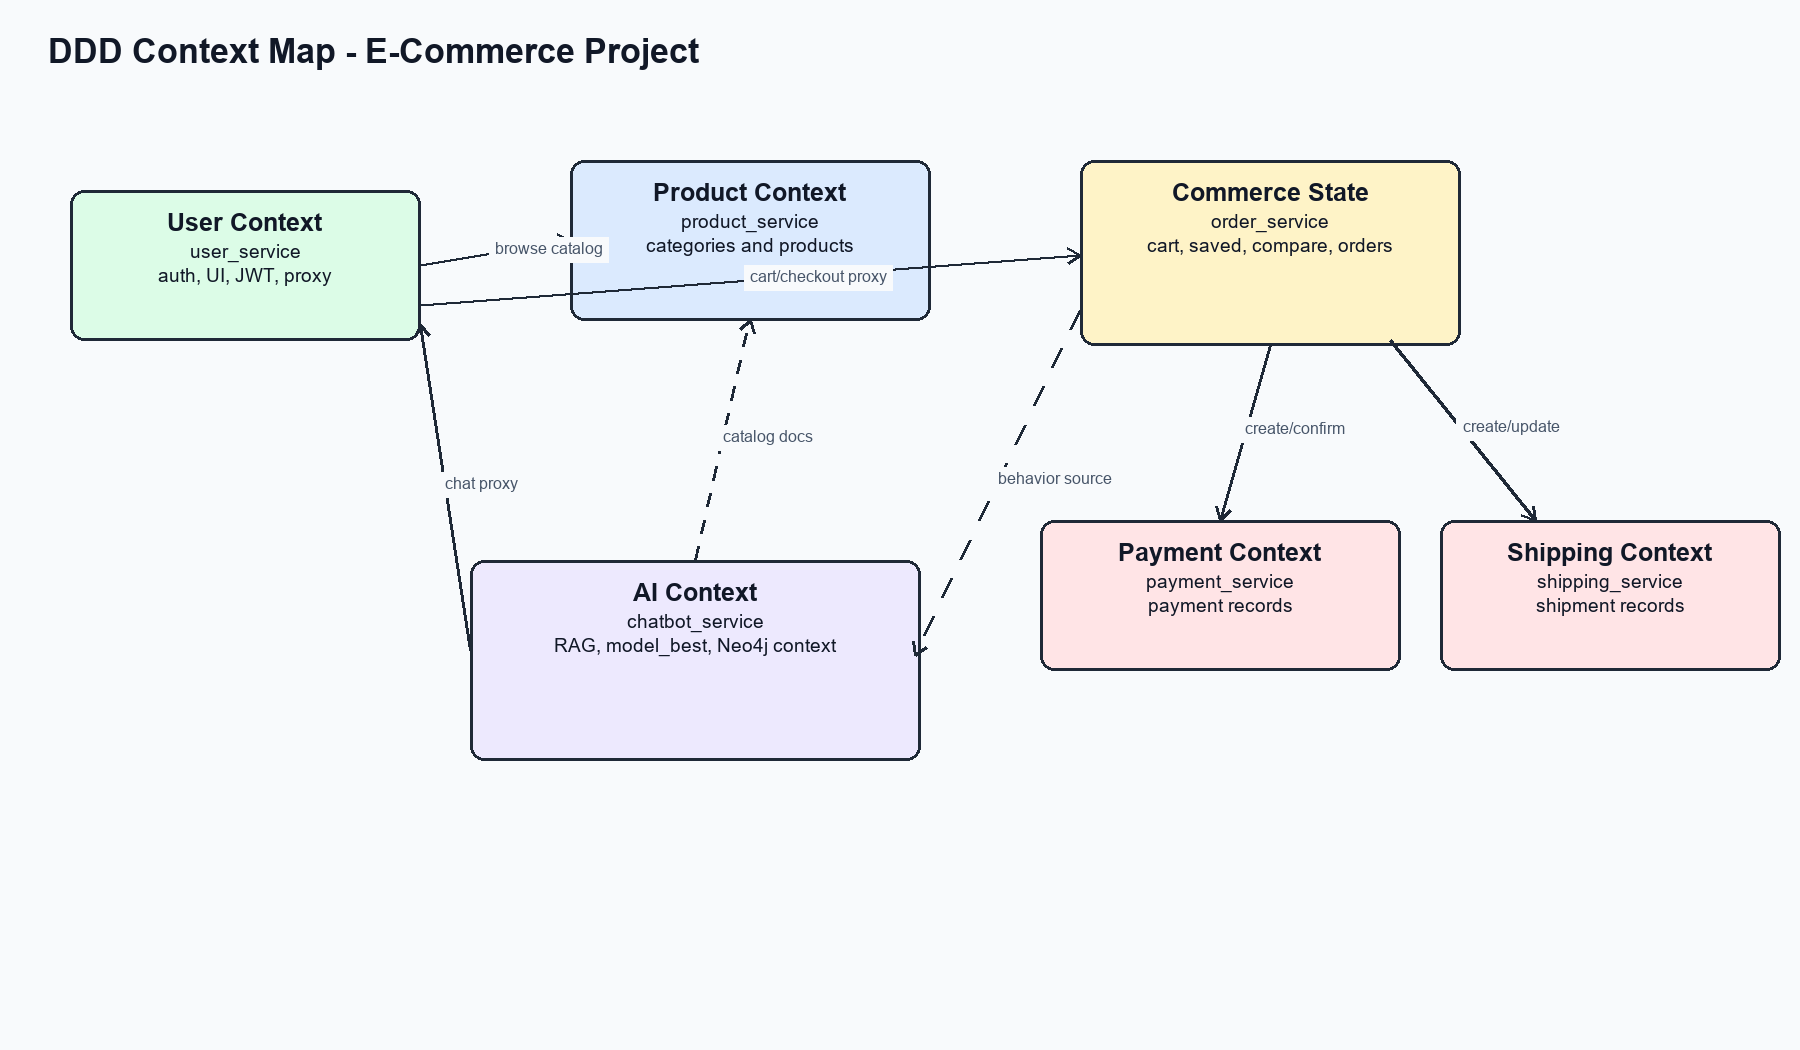
\includegraphics[width=0.95\linewidth]{final_diagram_images/ecom_context_map.png}
\caption{DDD context map for the target e-commerce system.}
\label{fig:ecom-context-map}
\end{figure}

\subsubsection{DDD in Microservices}

DDD is useful for microservices because one bounded context is often a good candidate for one microservice. This does not mean every class becomes a service. The goal is to group behavior and data that change together.

\subsection{Case Study: Healthcare (Practice Decomposition)}

\subsubsection{Problem Description}

Healthcare is used here only as a decomposition case study, not as the main project of the essay. The purpose is to practice DDD thinking in a domain that has multiple business capabilities, such as patient identity, appointment, medical record, billing, pharmacy, and notification.

\subsubsection{Step 1: Identify the Domain}

The domain is a healthcare service system. The core business goal is to help users receive healthcare services safely and traceably. The system may contain patient registration, appointment booking, medical record management, pharmacy support, billing, and notification.

\subsubsection{Step 2: Identify Bounded Contexts}

The healthcare domain can be decomposed into these bounded contexts:

\begin{itemize}
    \item Patient/User Context.
    \item Appointment Context.
    \item Medical Record Context.
    \item Pharmacy Context.
    \item Billing Context.
    \item Notification Context.
\end{itemize}

\subsubsection{Step 3: Decompose into Microservices}

\begin{figure}[H]
\centering
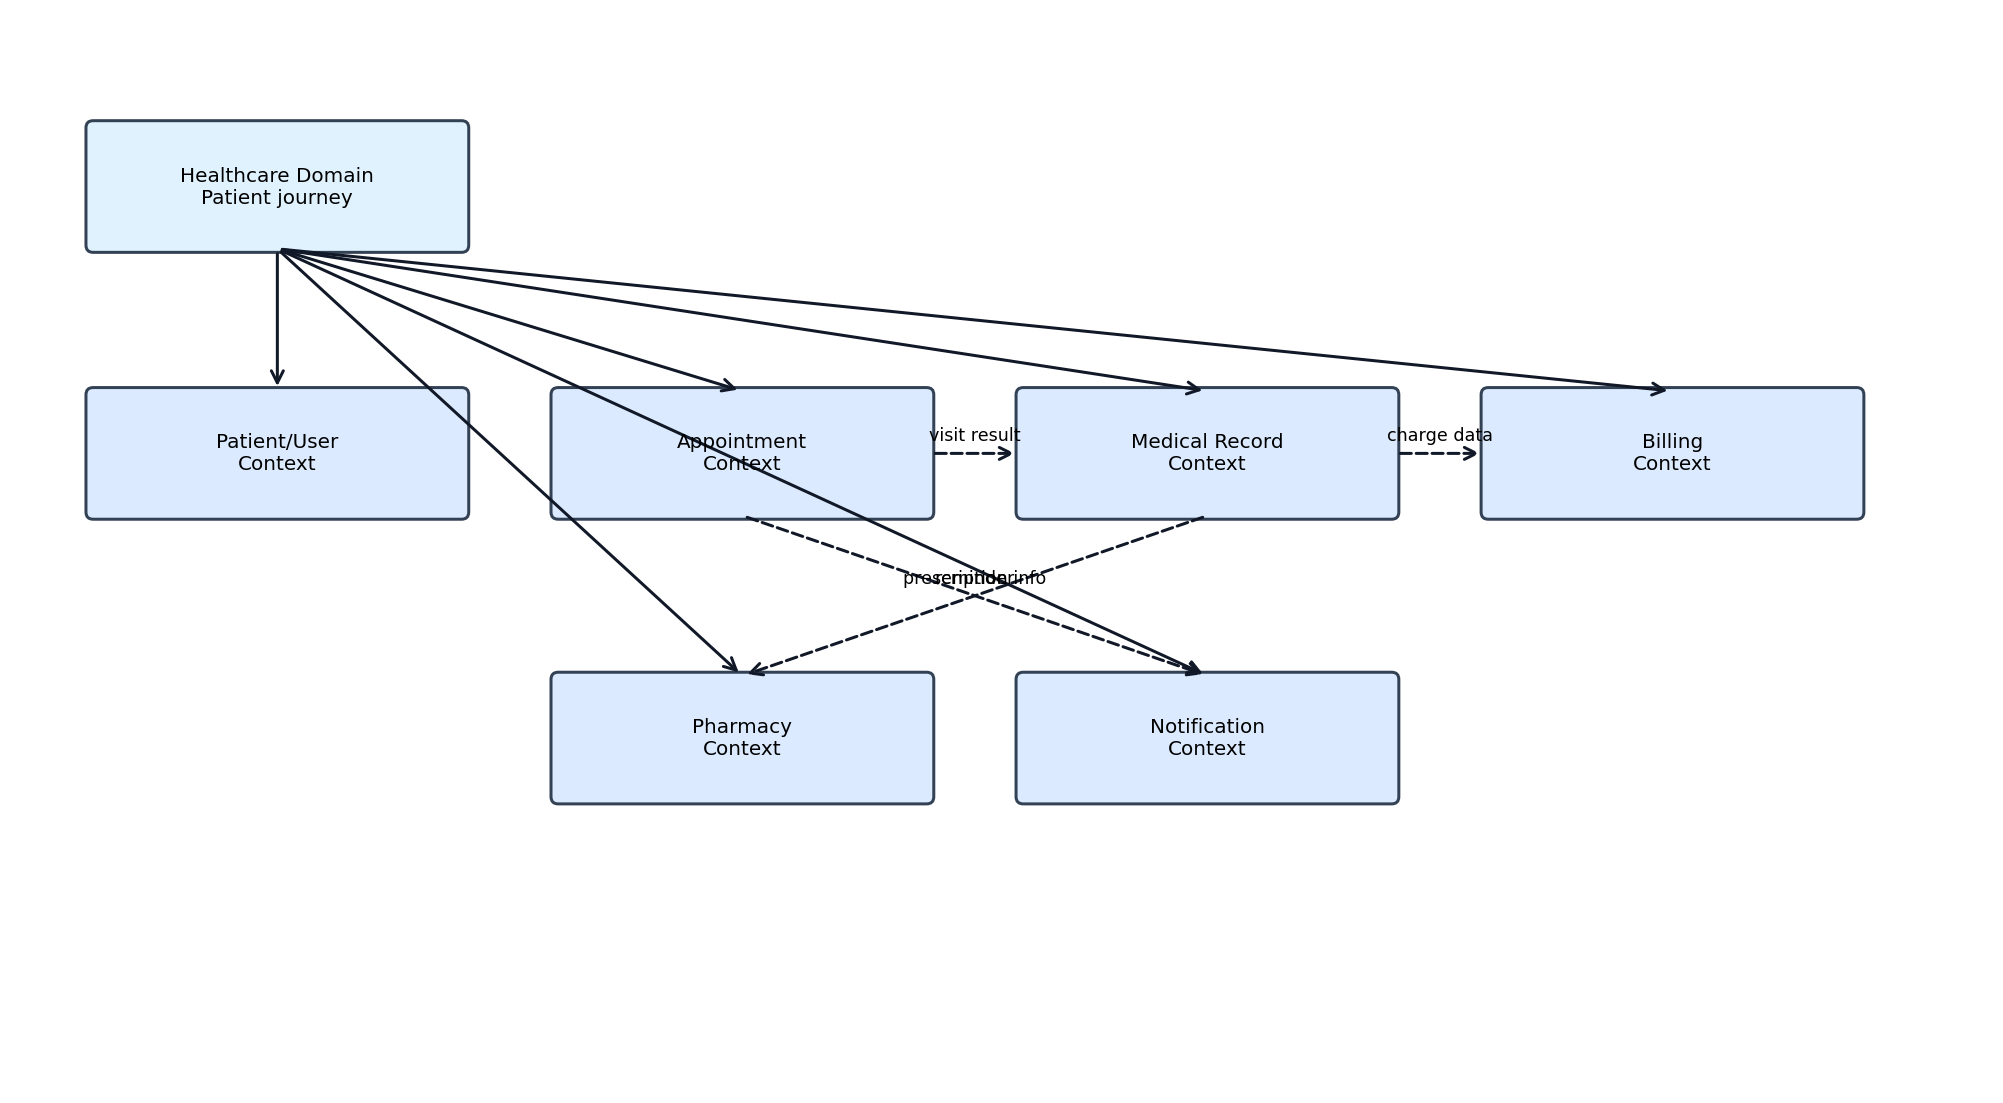
\includegraphics[width=0.92\linewidth]{final_diagram_images/healthcare_case_decomposition.png}
\caption{Healthcare case study decomposition for DDD practice.}
\label{fig:healthcare-case}
\end{figure}

Each context can become a service if it has enough independent business behavior. For example, appointment scheduling and billing should not share one database model because their business rules change for different reasons.

\subsubsection{Step 4: Identify Relationships}

The Appointment Context may call Notification to send reminders. The Medical Record Context may produce billing information. The Pharmacy Context may consume prescription-related information. These interactions should happen through APIs, not through direct database access.

\subsubsection{Example API}

\begin{lstlisting}[caption={Example healthcare API decomposition.}]
POST /api/patients/
POST /api/appointments/
GET  /api/medical-records/{patient_id}/
POST /api/pharmacy/dispense-requests/
POST /api/billing/invoices/
\end{lstlisting}

\subsection{Conclusion}

Monolithic architecture is suitable for simple early systems, but microservices are more appropriate when the system grows and the domain has clear boundaries. DDD provides a systematic way to identify those boundaries before creating services.

\section{Developing the Current E-Commerce Microservices System}

\subsection{Project Identification}

The real project used in this essay is the Docker-based Django commerce project in
\codepath{c:/Users/nguye/Desktop/kiemtra01}. The source evidence comes from
\codepath{README.md}, \codepath{docker-compose.yml}, \codepath{docker/gateway/nginx.conf},
and the service folders under \codepath{services/}. Unlike a purely theoretical design,
this project is already decomposed into six application services, one Nginx gateway,
shared infrastructure containers, and optional Neo4j graph storage for the AI service.

\begin{longtable}{p{0.22\linewidth}p{0.18\linewidth}p{0.18\linewidth}p{0.32\linewidth}}
\caption{Real service matrix from Docker Compose.}
\label{tab:real-service-matrix}\\
\toprule
\textbf{Service} & \textbf{Host/port} & \textbf{Database} & \textbf{Role}\\
\midrule
\endfirsthead
\toprule
\textbf{Service} & \textbf{Host/port} & \textbf{Database} & \textbf{Role}\\
\midrule
\endhead
\codepath{gateway} & \codepath{localhost:8080} & none & Public Nginx entrypoint.\\
\codepath{user\_service} & \codepath{8000}, \codepath{8003} debug & MySQL \codepath{user\_db} & Customer/staff UI, session auth, JWT auth, gateway metadata, chatbot proxy.\\
\codepath{product\_service} & \codepath{8001} debug & PostgreSQL \codepath{product\_db} & Catalog API, categories, products, seed data.\\
\codepath{order\_service} & internal only & MySQL \codepath{order\_db} & Cart, saved items, compare list, checkout, orders, shipping snapshot, analytics.\\
\codepath{payment\_service} & internal only & PostgreSQL \codepath{payment\_db} & Payment records and confirmation lifecycle.\\
\codepath{shipping\_service} & internal only & PostgreSQL \codepath{shipping\_db} & Shipment records and status lifecycle.\\
\codepath{chatbot\_service} & \codepath{8005} debug & PostgreSQL \codepath{chatbot\_db} & Chatbot, RAG, behavior model, Neo4j graph context.\\
\codepath{neo4j} & \codepath{7474}, \codepath{7687} & graph store & Optional behavior graph for chatbot context.\\
\bottomrule
\end{longtable}

\subsection{Requirement Identification}

\subsubsection{Functional Requirements}

The implemented system supports:

\begin{itemize}
    \item Customer registration, login, dashboard browsing, product detail, saved list, compare list, cart, checkout, orders, and chatbot UI.
    \item Staff login, dashboard, product management, customer inspection, order inspection, and shipping status updates.
    \item Catalog browsing across 10 categories and 100 seeded demo products from \codepath{services/product\_service/catalog/seed\_data.py}.
    \item Checkout orchestration in \codepath{order\_service}, with payment records delegated to \codepath{payment\_service} and shipment records delegated to \codepath{shipping\_service}.
    \item AI-assisted recommendations on dashboard/cart and chatbot replies through \codepath{chatbot\_service}.
\end{itemize}

\subsubsection{Non-functional Requirements}

\begin{itemize}
    \item \textbf{Deployability}: Docker Compose starts the gateway, services, MySQL, PostgreSQL, and Neo4j.
    \item \textbf{Boundary ownership}: every service owns its models and database; cross-service references are IDs or snapshots.
    \item \textbf{Stable public entrypoint}: Nginx stays on \codepath{8080}; direct service ports are only debug surfaces.
    \item \textbf{Security}: browser UI uses Django sessions; API auth uses JWT; internal service calls use \codepath{X-Internal-Key}.
    \item \textbf{Resilience}: chatbot still returns a rule-based/catalog response if the configured LLM or Neo4j graph is unavailable.
\end{itemize}

\subsection{DDD-Based System Decomposition}

\subsubsection{Bounded Contexts}

\begin{longtable}{p{0.24\linewidth}p{0.24\linewidth}p{0.42\linewidth}}
\caption{Real bounded contexts and service ownership.}
\label{tab:real-bounded-contexts}\\
\toprule
\textbf{Bounded context} & \textbf{Physical service} & \textbf{Evidence}\\
\midrule
\endfirsthead
\toprule
\textbf{Bounded context} & \textbf{Physical service} & \textbf{Evidence}\\
\midrule
\endhead
User and Web Edge & \codepath{user\_service} & \codepath{customer/urls.py}, \codepath{staff/urls.py}, \codepath{customer/api\_auth.py}\\
Catalog & \codepath{product\_service} & \codepath{catalog/models.py}, \codepath{catalog/urls.py}, \codepath{catalog/seed\_data.py}\\
Cart, Saved, Compare, Order & \codepath{order\_service} & \codepath{orders/models.py}; cart is a module inside order service, not a separate container.\\
Payment & \codepath{payment\_service} & \codepath{payments/models.py}, \codepath{payments/urls.py}\\
Shipping & \codepath{shipping\_service} & \codepath{shipments/models.py}, \codepath{shipments/urls.py}\\
AI Consultation & \codepath{chatbot\_service} & \codepath{chatbot/services.py}, \codepath{chatbot/behavior\_ai.py}, \codepath{chatbot/rag\_kb.py}\\
\bottomrule
\end{longtable}

\begin{figure}[H]
\centering
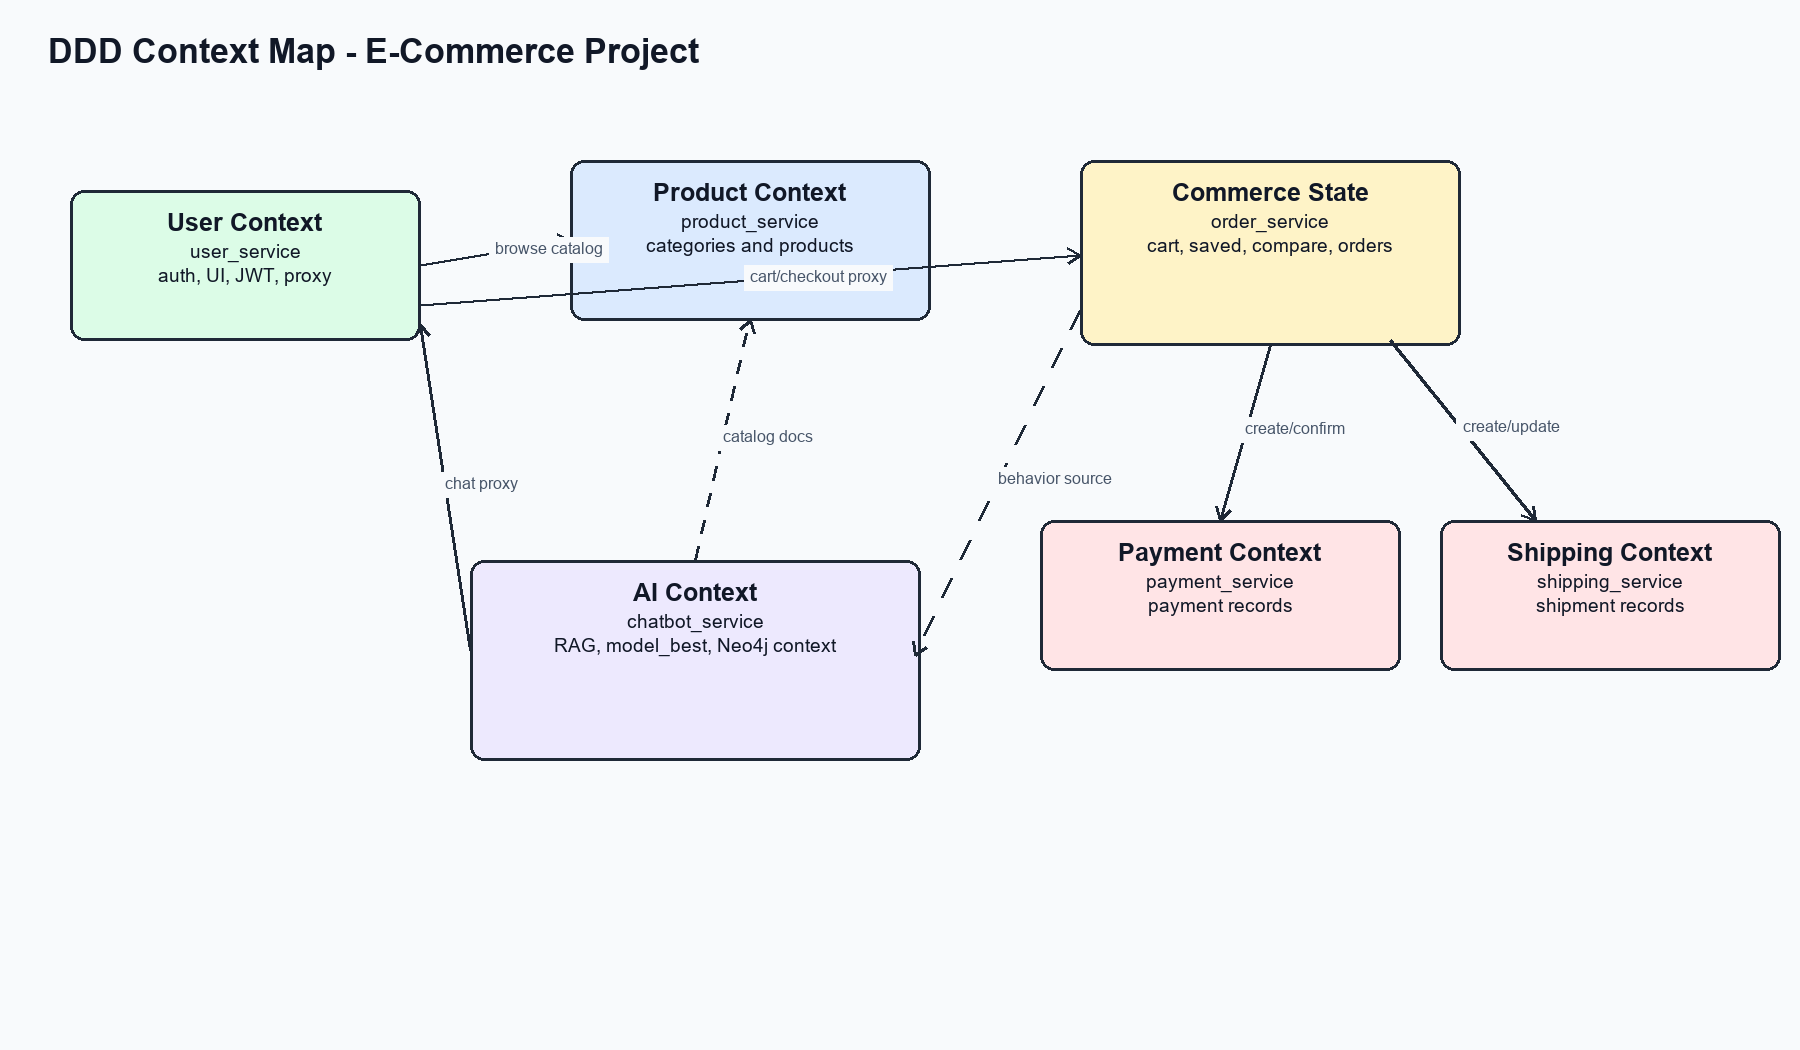
\includegraphics[width=0.98\linewidth]{final_diagram_images/ecom_context_map.png}
\caption{DDD context map for the current e-commerce system.}
\label{fig:ecom-context-map-real}
\end{figure}

The important design point is that \codepath{cart} is a bounded capability but not a separate physical service in this repository. It is implemented inside \codepath{order\_service} through \codepath{CartItem}, \codepath{SavedItem}, and \codepath{CompareItem}. This is a practical service-boundary choice: all mutable commerce state changes together and is protected by the same internal key.

\subsection{Product Service Design}

\subsubsection{Model Evidence}

The catalog model is implemented in \codepath{services/product\_service/catalog/models.py}. A category owns many products, and deleting a category is protected by \codepath{on\_delete=models.PROTECT}.

\begin{lstlisting}[language=Python,caption={Real product service model excerpt.}]
class Category(models.Model):
    name = models.CharField(max_length=120, unique=True)
    slug = models.SlugField(max_length=120, unique=True)
    description = models.TextField(blank=True)
    sort_order = models.PositiveIntegerField(default=0)
    is_active = models.BooleanField(default=True)

class Product(models.Model):
    category = models.ForeignKey(Category, on_delete=models.PROTECT,
                                 related_name="products")
    name = models.CharField(max_length=255)
    brand = models.CharField(max_length=120, default="Generic")
    price = models.DecimalField(max_digits=12, decimal_places=2)
    stock = models.PositiveIntegerField(default=0)
\end{lstlisting}

\subsubsection{API Evidence}

\codepath{catalog/urls.py} registers DRF routes for \codepath{categories} and \codepath{products}. The Nginx gateway exposes these as \codepath{/api/categories/} and \codepath{/api/products/}.

\begin{lstlisting}[caption={Product service API routes.}]
GET    /api/categories/
GET    /api/products/
GET    /api/products/{id}/
POST   /api/products/          # staff key required
PUT    /api/products/{id}/     # staff key required
DELETE /api/products/{id}/     # staff key required
\end{lstlisting}

\subsection{User Service Design}

\subsubsection{Authentication Model}

The project uses Django's built-in \codepath{auth\_user} table instead of a custom role model. Role is derived from \codepath{is\_staff} and \codepath{is\_superuser} in \codepath{customer/auth\_rules.py}. The same service also owns customer/staff templates, editorial content, JWT API auth, and the customer-facing chatbot proxy.

\begin{lstlisting}[caption={JWT auth API in user\_service.}]
POST /api/auth/register/
POST /api/auth/token/
POST /api/auth/token/refresh/
GET  /api/auth/me/
\end{lstlisting}

Browser routes such as \codepath{/customer/login/}, \codepath{/customer/dashboard/}, \codepath{/customer/cart/}, and \codepath{/staff/orders/} remain stable. Customer and staff sessions use separate cookie names, so both roles can be demonstrated in one browser.

\subsection{Cart and Order Service Design}

\subsubsection{Cart Model}

Cart state is stored in \codepath{order\_service}. There is no separate \codepath{cart\_service} container and no physical \codepath{cart} table. Instead, \codepath{CartItem} is user-scoped by \codepath{user\_id} and keeps a product snapshot so the order database never directly joins the product database.

\begin{lstlisting}[language=Python,caption={Real cart and snapshot model excerpt.}]
class ProductSnapshotMixin(models.Model):
    category_slug = models.SlugField(max_length=120, blank=True)
    category_name = models.CharField(max_length=120, blank=True)
    product_id = models.PositiveIntegerField(default=0)
    product_name = models.CharField(max_length=255)
    product_brand = models.CharField(max_length=120, blank=True)
    unit_price = models.DecimalField(max_digits=12, decimal_places=2)

class CartItem(ProductSnapshotMixin):
    user_id = models.PositiveIntegerField(db_index=True)
    quantity = models.PositiveIntegerField(default=1)
\end{lstlisting}

\subsubsection{Order Model and Workflow}

\begin{lstlisting}[language=Python,caption={Real order model excerpt.}]
class Order(models.Model):
    user_id = models.PositiveIntegerField(db_index=True)
    total_amount = models.DecimalField(max_digits=12, decimal_places=2)
    payment_status = models.CharField(max_length=20, default="pending")
    shipping_status = models.CharField(max_length=20, default="pending")
    source = models.CharField(max_length=20, default="live")

class OrderItem(ProductSnapshotMixin):
    order = models.ForeignKey(Order, on_delete=models.CASCADE,
                              related_name="items")
    quantity = models.PositiveIntegerField(default=1)
\end{lstlisting}

\codepath{orders/urls.py} exposes \codepath{/api/cart/}, \codepath{/api/checkout/}, \codepath{/api/orders/}, \codepath{/api/orders/\{id\}/pay/}, \codepath{/api/staff/orders/}, and internal behavior-source APIs. All order endpoints require an internal key when called from other services.

\subsection{Payment and Shipping Services}

\subsubsection{Payment Service}

\begin{lstlisting}[language=Python,caption={Real payment model excerpt.}]
class Payment(models.Model):
    order_id = models.PositiveIntegerField(unique=True)
    user_id = models.PositiveIntegerField(db_index=True)
    amount = models.DecimalField(max_digits=12, decimal_places=2)
    status = models.CharField(max_length=20, default="pending")
    paid_at = models.DateTimeField(null=True, blank=True)
\end{lstlisting}

Payment status can be \codepath{pending}, \codepath{paid}, \codepath{failed}, or \codepath{cancelled}. The API includes \codepath{/api/payments/}, \codepath{/api/payments/by-order/\{order\_id\}/}, \codepath{/api/payments/\{id\}/confirm/}, and \codepath{/api/payments/\{id\}/cancel/}.

\subsubsection{Shipping Service}

\begin{lstlisting}[language=Python,caption={Real shipment model excerpt.}]
class Shipment(models.Model):
    order_id = models.PositiveIntegerField(unique=True)
    user_id = models.PositiveIntegerField(db_index=True)
    recipient_name = models.CharField(max_length=120)
    address_line = models.CharField(max_length=255)
    status = models.CharField(max_length=20, default="pending")
\end{lstlisting}

Shipping status can move through \codepath{pending}, \codepath{preparing}, \codepath{shipped}, \codepath{delivered}, and \codepath{cancelled}. Invalid transitions are rejected in \codepath{Shipment.can\_update\_status()}.

\subsection{Class Diagram and Data Model}

\begin{figure}[H]
\centering
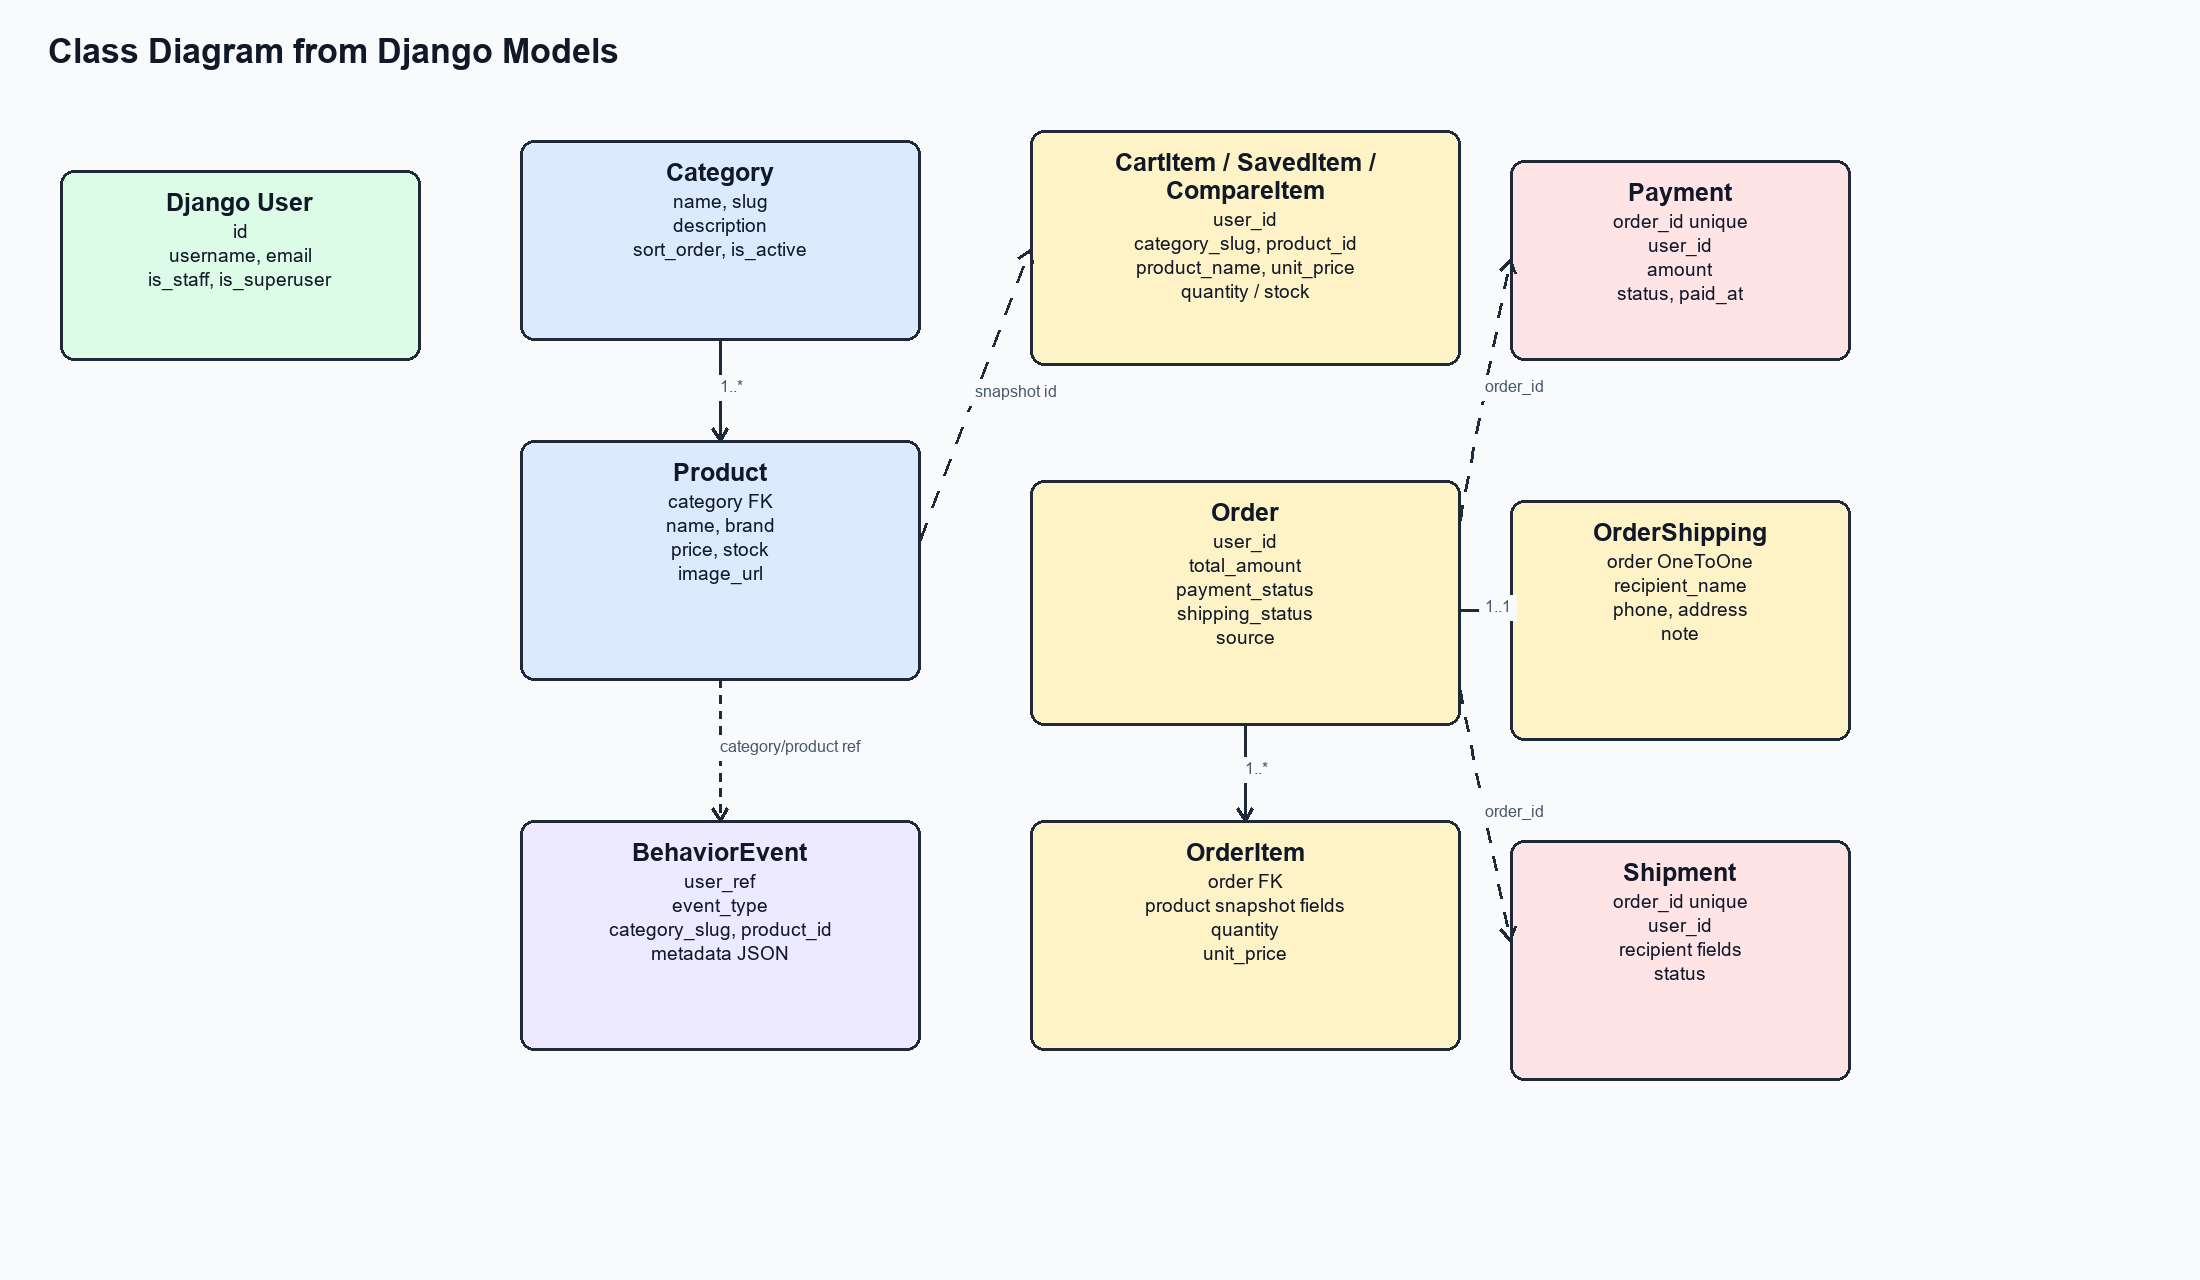
\includegraphics[width=0.98\linewidth]{final_diagram_images/ecom_class_diagram.png}
\caption{Class diagram from real Django models.}
\label{fig:ecom-class-diagram}
\end{figure}

\begin{figure}[H]
\centering
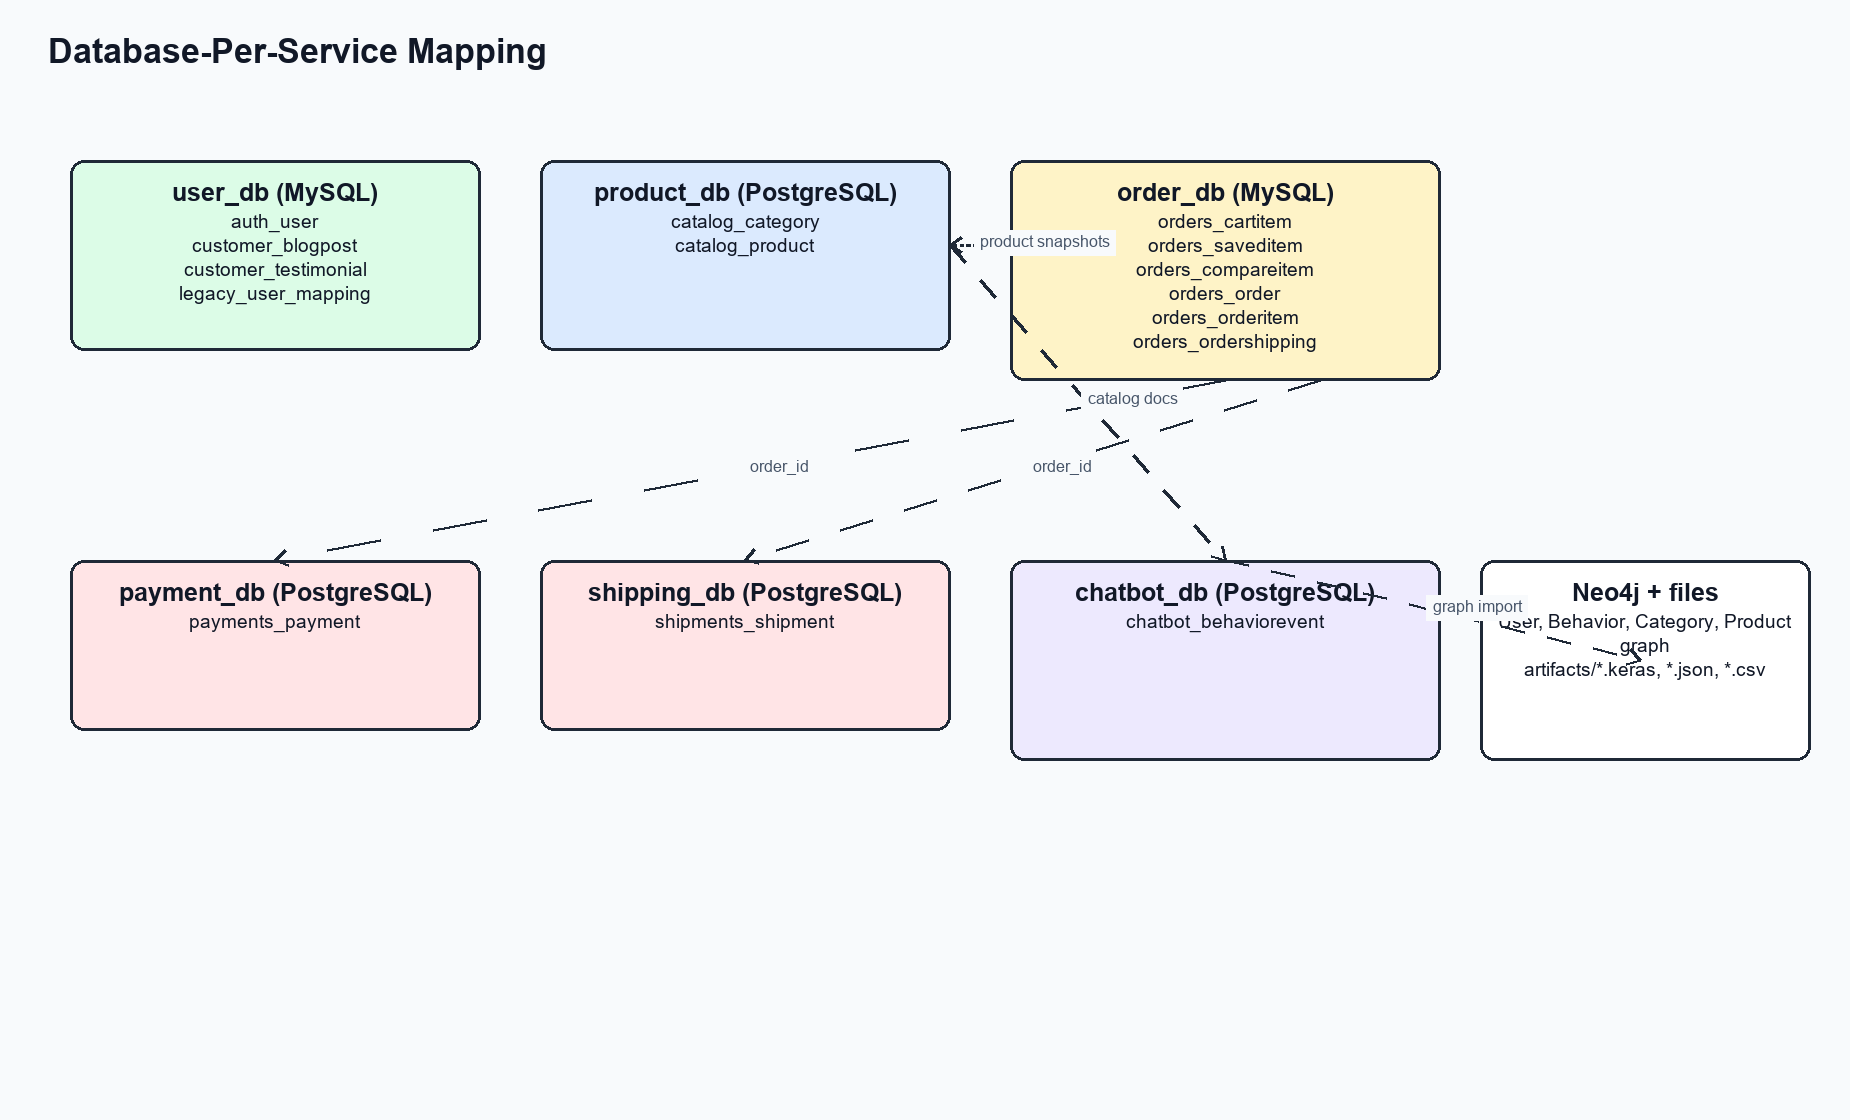
\includegraphics[width=0.98\linewidth]{final_diagram_images/ecom_database_mapping.png}
\caption{Database-per-service mapping from Docker Compose and Django settings.}
\label{fig:ecom-db-mapping}
\end{figure}

The following diagrams are exported from Visual Paradigm and included as the final design evidence. They provide a more detailed view than the summarized report diagrams above: the class diagram shows the main domain objects and service ownership, while the ORM and ERD diagrams show how those objects are persisted across the service databases.

\begin{figure}[H]
\centering
\diagramimage[width=0.98\linewidth]{final_diagram_images/Class_Diagram_E_Commerce}
\caption{Visual Paradigm class diagram for the e-commerce microservices system.}
\label{fig:vp-class-diagram}
\end{figure}

\begin{figure}[H]
\centering
\diagramimage[width=0.98\linewidth]{final_diagram_images/DataModel_ORM}
\caption{Visual Paradigm ORM data model for the e-commerce system.}
\label{fig:vp-orm-diagram}
\end{figure}

\begin{figure}[H]
\centering
\diagramimage[width=0.98\linewidth]{final_diagram_images/DataModel_ORM_ERD}
\caption{Visual Paradigm ERD view of the ORM data model.}
\label{fig:vp-erd-diagram}
\end{figure}

\subsection{Database Design}

\subsubsection{Database Engines}

The database engines are defined in each service's \codepath{config/settings.py}. \codepath{user\_service} and \codepath{order\_service} use MySQL. \codepath{product\_service}, \codepath{payment\_service}, \codepath{shipping\_service}, and \codepath{chatbot\_service} use PostgreSQL. The initialization scripts are \codepath{docker/mysql-init/01-create-databases.sql} and \codepath{docker/postgres-init/01-create-databases.sql}.

\begin{longtable}{p{0.25\linewidth}p{0.23\linewidth}p{0.42\linewidth}}
\caption{Main database tables in the real project.}
\label{tab:real-db-tables}\\
\toprule
\textbf{Database} & \textbf{Engine} & \textbf{Main tables}\\
\midrule
\endfirsthead
\toprule
\textbf{Database} & \textbf{Engine} & \textbf{Main tables}\\
\midrule
\endhead
\codepath{user\_db} & MySQL & \codepath{auth\_user}, \codepath{customer\_blogpost}, \codepath{customer\_testimonial}, \codepath{customer\_legacyusermapping}\\
\codepath{product\_db} & PostgreSQL & \codepath{catalog\_category}, \codepath{catalog\_product}\\
\codepath{order\_db} & MySQL & \codepath{orders\_cartitem}, \codepath{orders\_saveditem}, \codepath{orders\_compareitem}, \codepath{orders\_order}, \codepath{orders\_orderitem}, \codepath{orders\_ordershipping}\\
\codepath{payment\_db} & PostgreSQL & \codepath{payments\_payment}\\
\codepath{shipping\_db} & PostgreSQL & \codepath{shipments\_shipment}\\
\codepath{chatbot\_db} & PostgreSQL & \codepath{chatbot\_behaviorevent}\\
\bottomrule
\end{longtable}

\subsubsection{SQL Schema Summary}

The following SQL summarizes the report-level schema. Names are normalized for readability; the real Django tables use app prefixes such as \codepath{catalog\_product} and \codepath{orders\_cartitem}. The logical \codepath{cart} table is included to explain the cart aggregate, while the current implementation stores the active cart directly as user-scoped \codepath{orders\_cartitem} rows.

\begin{lstlisting}[language=SQL,caption={Database schema summary for the e-commerce system.}]
CREATE TABLE category (
    id BIGSERIAL PRIMARY KEY,
    name VARCHAR(120) NOT NULL UNIQUE,
    slug VARCHAR(120) NOT NULL UNIQUE,
    description TEXT NOT NULL DEFAULT '',
    sort_order INTEGER NOT NULL DEFAULT 0,
    is_active BOOLEAN NOT NULL DEFAULT TRUE
);

CREATE TABLE product (
    id BIGSERIAL PRIMARY KEY,
    category_id BIGINT NOT NULL REFERENCES category(id),
    name VARCHAR(255) NOT NULL,
    brand VARCHAR(120) NOT NULL DEFAULT 'Generic',
    description TEXT NOT NULL DEFAULT '',
    image_url VARCHAR(200) NOT NULL DEFAULT '',
    price DECIMAL(12,2) NOT NULL,
    stock INTEGER NOT NULL DEFAULT 0,
    created_at TIMESTAMP NOT NULL,
    updated_at TIMESTAMP NOT NULL,
    UNIQUE (category_id, name, brand)
);

CREATE TABLE user_account (
    id BIGINT PRIMARY KEY,
    username VARCHAR(150) NOT NULL UNIQUE,
    email VARCHAR(254) NOT NULL,
    password VARCHAR(128) NOT NULL,
    is_staff BOOLEAN NOT NULL DEFAULT FALSE,
    is_superuser BOOLEAN NOT NULL DEFAULT FALSE
);

CREATE TABLE cart (
    id BIGINT PRIMARY KEY,
    user_id BIGINT NOT NULL,
    created_at TIMESTAMP NOT NULL,
    updated_at TIMESTAMP NOT NULL
);

CREATE TABLE cart_item (
    id BIGINT PRIMARY KEY,
    user_id BIGINT NOT NULL,
    category_slug VARCHAR(120) NOT NULL,
    category_name VARCHAR(120) NOT NULL,
    product_id BIGINT NOT NULL,
    product_name VARCHAR(255) NOT NULL,
    product_brand VARCHAR(120) NOT NULL,
    unit_price DECIMAL(12,2) NOT NULL,
    quantity INTEGER NOT NULL DEFAULT 1,
    UNIQUE (user_id, category_slug, product_id)
);

CREATE TABLE orders (
    id BIGINT PRIMARY KEY,
    user_id BIGINT NOT NULL,
    total_amount DECIMAL(12,2) NOT NULL,
    payment_status VARCHAR(20) NOT NULL DEFAULT 'pending',
    shipping_status VARCHAR(20) NOT NULL DEFAULT 'pending',
    source VARCHAR(20) NOT NULL DEFAULT 'live',
    source_order_id BIGINT NULL,
    paid_at TIMESTAMP NULL,
    created_at TIMESTAMP NOT NULL,
    updated_at TIMESTAMP NOT NULL
);

CREATE TABLE order_item (
    id BIGINT PRIMARY KEY,
    order_id BIGINT NOT NULL REFERENCES orders(id),
    category_slug VARCHAR(120) NOT NULL,
    product_id BIGINT NOT NULL,
    product_name VARCHAR(255) NOT NULL,
    product_brand VARCHAR(120) NOT NULL,
    unit_price DECIMAL(12,2) NOT NULL,
    quantity INTEGER NOT NULL DEFAULT 1
);

CREATE TABLE payment (
    id BIGINT PRIMARY KEY,
    order_id BIGINT NOT NULL UNIQUE,
    user_id BIGINT NOT NULL,
    amount DECIMAL(12,2) NOT NULL,
    status VARCHAR(20) NOT NULL DEFAULT 'pending',
    paid_at TIMESTAMP NULL,
    created_at TIMESTAMP NOT NULL,
    updated_at TIMESTAMP NOT NULL
);

CREATE TABLE shipment (
    id BIGINT PRIMARY KEY,
    order_id BIGINT NOT NULL UNIQUE,
    user_id BIGINT NOT NULL,
    recipient_name VARCHAR(120) NOT NULL,
    phone VARCHAR(40) NOT NULL,
    address_line VARCHAR(255) NOT NULL,
    city_or_region VARCHAR(120) NOT NULL,
    postal_code VARCHAR(40) NOT NULL,
    country VARCHAR(120) NOT NULL,
    status VARCHAR(20) NOT NULL DEFAULT 'pending',
    created_at TIMESTAMP NOT NULL,
    updated_at TIMESTAMP NOT NULL
);
\end{lstlisting}

\subsection{Conclusion}

The current project follows microservice decomposition in a pragmatic way. It has six application services rather than a separate service for every subdomain. The cart capability is grouped with order state, while payment, shipping, catalog, user/auth/UI, and AI remain independently deployable services with their own databases.

\section{AI Service for Product Consultation}

\subsection{Goal}

The AI capability is implemented by \codepath{chatbot\_service}. It supports product consultation, recommendation ranking, RAG citations, behavior persistence, optional Neo4j graph context, and fallback responses when LLM access is unavailable.

\subsection{AI Service Architecture}

\begin{figure}[H]
\centering
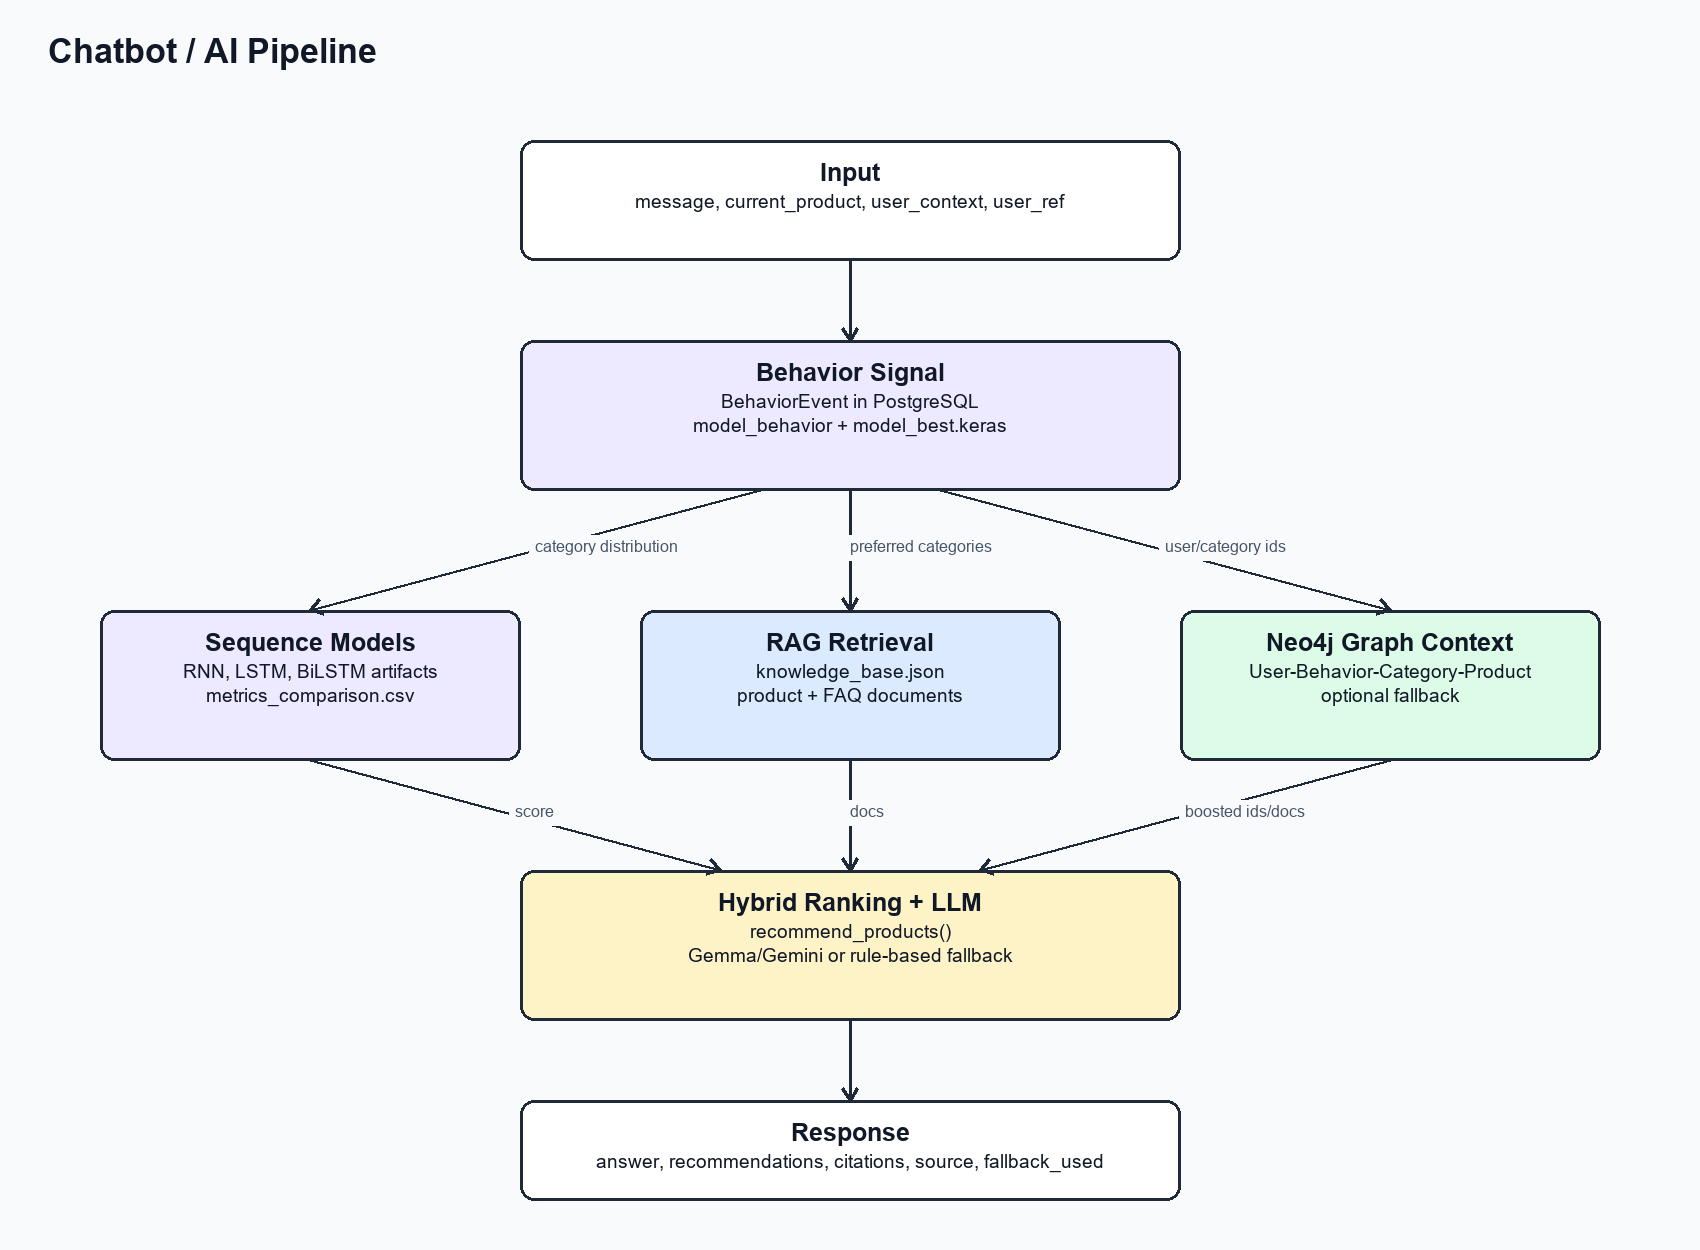
\includegraphics[width=0.92\linewidth]{final_diagram_images/ecom_ai_pipeline.png}
\caption{Real chatbot and AI recommendation pipeline.}
\label{fig:ecom-ai-pipeline}
\end{figure}

\subsection{Behavior Data}

\codepath{chatbot/models.py} defines \codepath{BehaviorEvent}. It records \codepath{user\_ref}, event type, category slug, product id, JSON metadata, and timestamp. The main recovery path is \codepath{user\_service}'s \codepath{backfill\_chatbot\_behavior} command, which can rebuild behavior input from order history.

\begin{lstlisting}[language=Python,caption={Real chatbot behavior model.}]
class BehaviorEvent(models.Model):
    user_ref = models.CharField(max_length=120, db_index=True)
    event_type = models.CharField(max_length=40)
    category_slug = models.CharField(max_length=120, blank=True)
    product_id = models.PositiveIntegerField(default=0)
    metadata = models.JSONField(default=dict, blank=True)
    created_at = models.DateTimeField(auto_now_add=True)
\end{lstlisting}

\subsection{Sequence Models: RNN, LSTM, and BiLSTM}

The artifact directory \codepath{services/chatbot\_service/chatbot/artifacts} contains trained model artifacts: \codepath{model\_rnn.keras}, \codepath{model\_lstm.keras}, \codepath{model\_bilstm.keras}, and \codepath{model\_best.keras}. The file \codepath{metrics\_comparison.csv} records the comparison.

\begin{table}[H]
\centering
\caption{AI model metrics from metrics\_comparison.csv.}
\label{tab:ai-model-metrics}
\begin{tabular}{lrrrrr}
\toprule
\textbf{Model} & \textbf{Accuracy} & \textbf{Macro F1} & \textbf{Params} & \textbf{Best epoch} & \textbf{Best val acc.}\\
\midrule
RNN & 0.999201 & 0.999410 & 11192 & 7 & 0.996697\\
LSTM & 0.999201 & 0.999410 & 29432 & 4 & 0.996697\\
BiLSTM & 0.999201 & 0.999410 & 57848 & 2 & 0.997523\\
\bottomrule
\end{tabular}
\end{table}

The runtime loads \codepath{model\_best.keras}, \codepath{label\_encoder.json}, and \codepath{tokenizer\_or\_vocab.json}. In the current artifacts, RNN is marked as the selected best model, while LSTM and BiLSTM are still present as trained evidence.

\subsection{Knowledge Graph with Neo4j}

Neo4j is optional and configured through \codepath{NEO4J\_URI}, \codepath{NEO4J\_USERNAME}, \codepath{NEO4J\_PASSWORD}, and \codepath{NEO4J\_DATABASE}. The importer in \codepath{chatbot/behavior\_graph.py} creates User, Behavior, Category, and Product nodes, plus relationships such as \codepath{PERFORMED}, \codepath{IN\_CATEGORY}, \codepath{ON\_PRODUCT}, \codepath{BELONGS\_TO}, and \codepath{PREFERS}.

\begin{lstlisting}[caption={Neo4j graph import relationship excerpt.}]
MERGE (u)-[:PERFORMED]->(b)
MERGE (b)-[:IN_CATEGORY]->(c)
MERGE (b)-[:ON_PRODUCT]->(p)
MERGE (p)-[:BELONGS_TO]->(c)
MERGE (u)-[pref:PREFERS]->(c)
\end{lstlisting}

If Neo4j is unavailable, \codepath{BehaviorGraphRetriever} returns an unavailable context and the chatbot continues with RAG and catalog ranking.

\subsection{RAG and Recommendation Flow}

\codepath{chatbot/rag\_kb.py} builds \codepath{knowledge\_base.json} from FAQ content and product documents fetched from \codepath{product\_service}. Retrieval uses token overlap, category preference, stock status, current product context, and behavior preference signals. The service also calls the live catalog API to build recommendation cards.

\begin{lstlisting}[caption={Chatbot API response contract.}]
POST /api/chat/reply/

Response fields:
answer
recommendations
citations
source
fallback_used
error_code
\end{lstlisting}

\subsection{Deployment Evidence}

The chatbot service is a Django service on internal port \codepath{8000} and host debug port \codepath{8005}. Docker Compose bind-mounts \codepath{./services/chatbot\_service/chatbot/artifacts} into the container, so generated knowledge bases, model files, metrics, and graph images are preserved outside the container.

\subsection{AI Evidence Checklist}

\begin{itemize}
    \item LSTM artifacts exist: \codepath{model\_lstm.keras}, \codepath{history\_lstm.png}, \codepath{confusion\_matrix\_lstm.png}.
    \item Neo4j graph code exists in \codepath{behavior\_graph.py} and demo evidence exists in \codepath{behavior\_graph\_demo.svg}.
    \item RAG file knowledge base exists in \codepath{knowledge\_base.json}.
    \item Chatbot API exists at \codepath{/api/chat/reply/}.
    \item Recommendation output is returned inside the chatbot response as \codepath{recommendations}.
    \item Screenshots are stored under \codepath{docs/evidence/screenshots/}.
\end{itemize}

\subsection{Conclusion}

The AI service is not a separate notebook-only experiment. It is wired into the running commerce system through \codepath{chatbot\_service}, called by \codepath{user\_service}, and backed by PostgreSQL behavior events, file-based RAG/model artifacts, optional Neo4j graph context, and live product-service data.

\section{Building the Complete System}

\subsection{Overall Architecture}

The complete system is deployed through Docker Compose. The public entrypoint is the Nginx gateway on \codepath{http://localhost:8080/}. The browser primarily uses gateway routes and customer/staff pages from \codepath{user\_service}; direct ports \codepath{8000}, \codepath{8001}, \codepath{8003}, and \codepath{8005} are debug surfaces.

\begin{figure}[H]
\centering
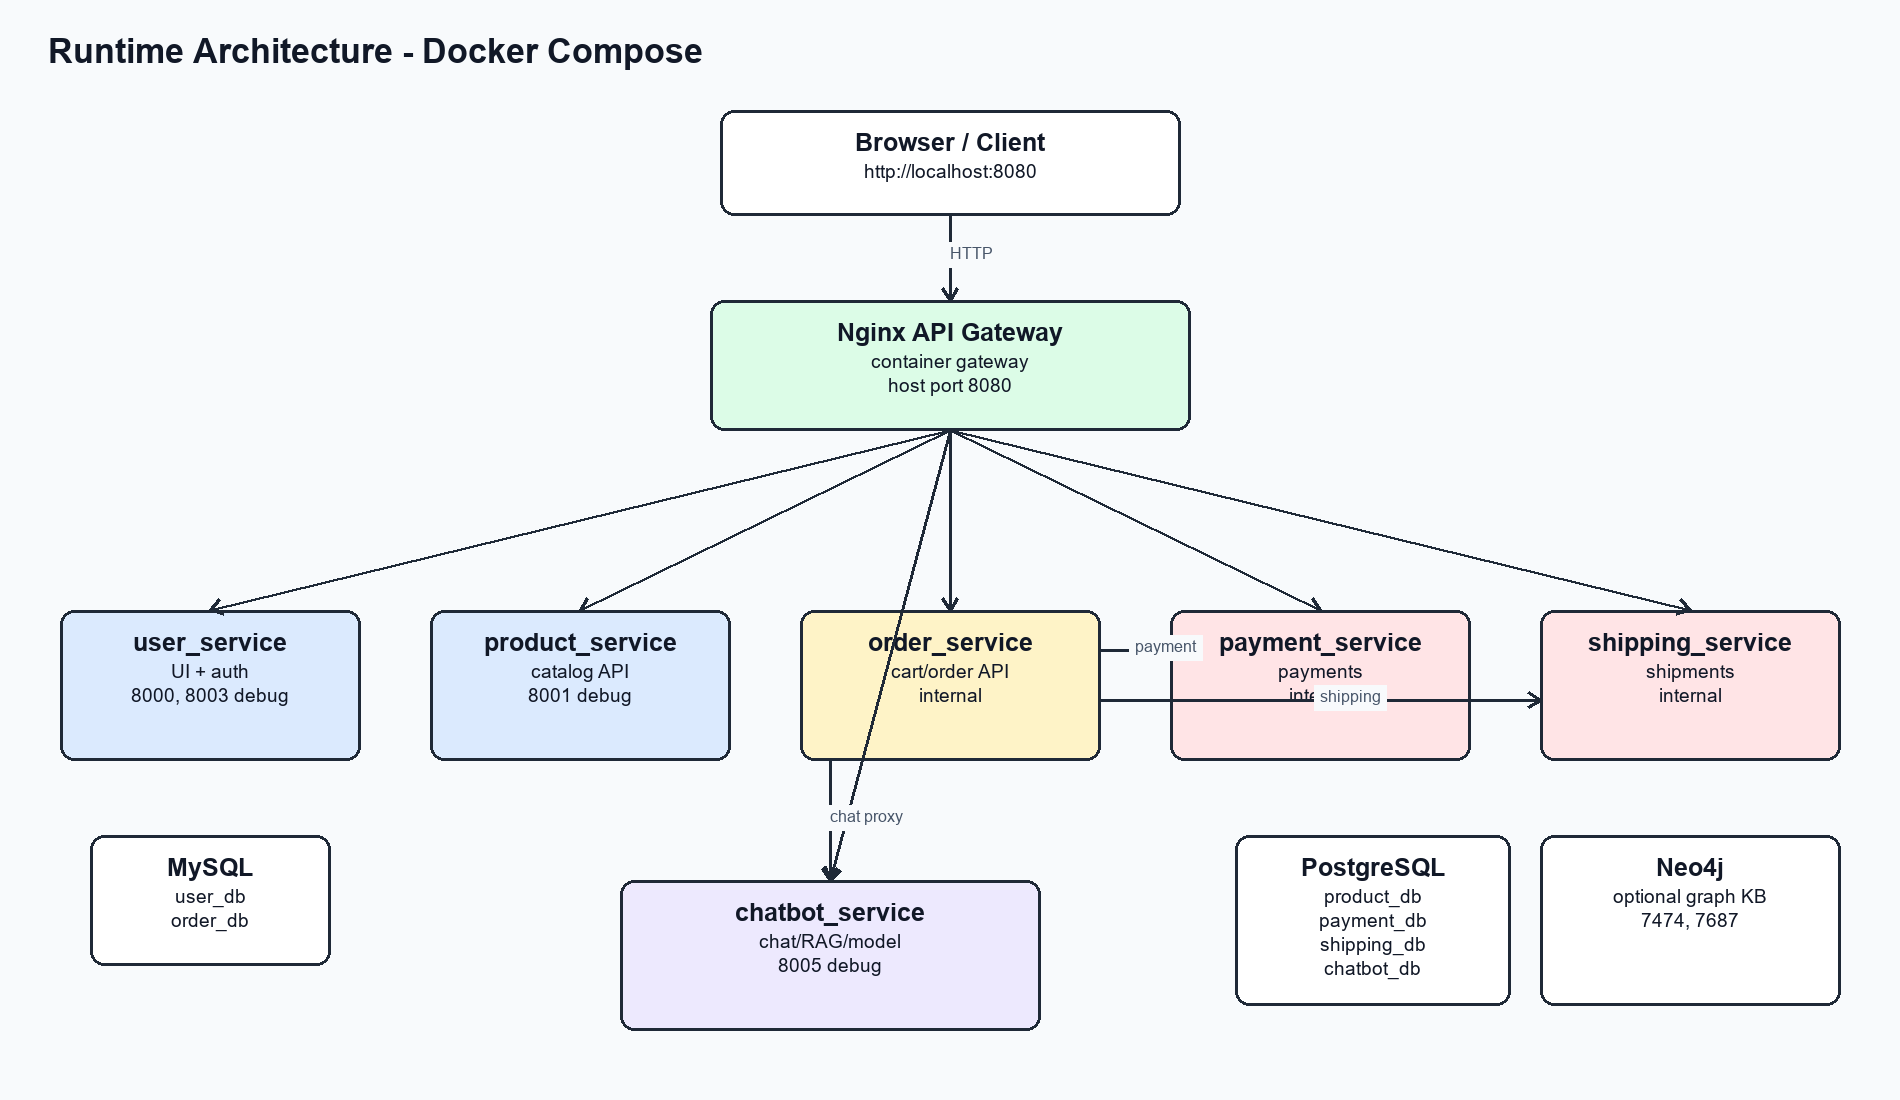
\includegraphics[width=0.98\linewidth]{final_diagram_images/ecom_system_architecture.png}
\caption{Runtime architecture of the real Docker Compose system.}
\label{fig:ecom-system-architecture}
\end{figure}

\subsection{API Gateway Routing}

\begin{figure}[H]
\centering
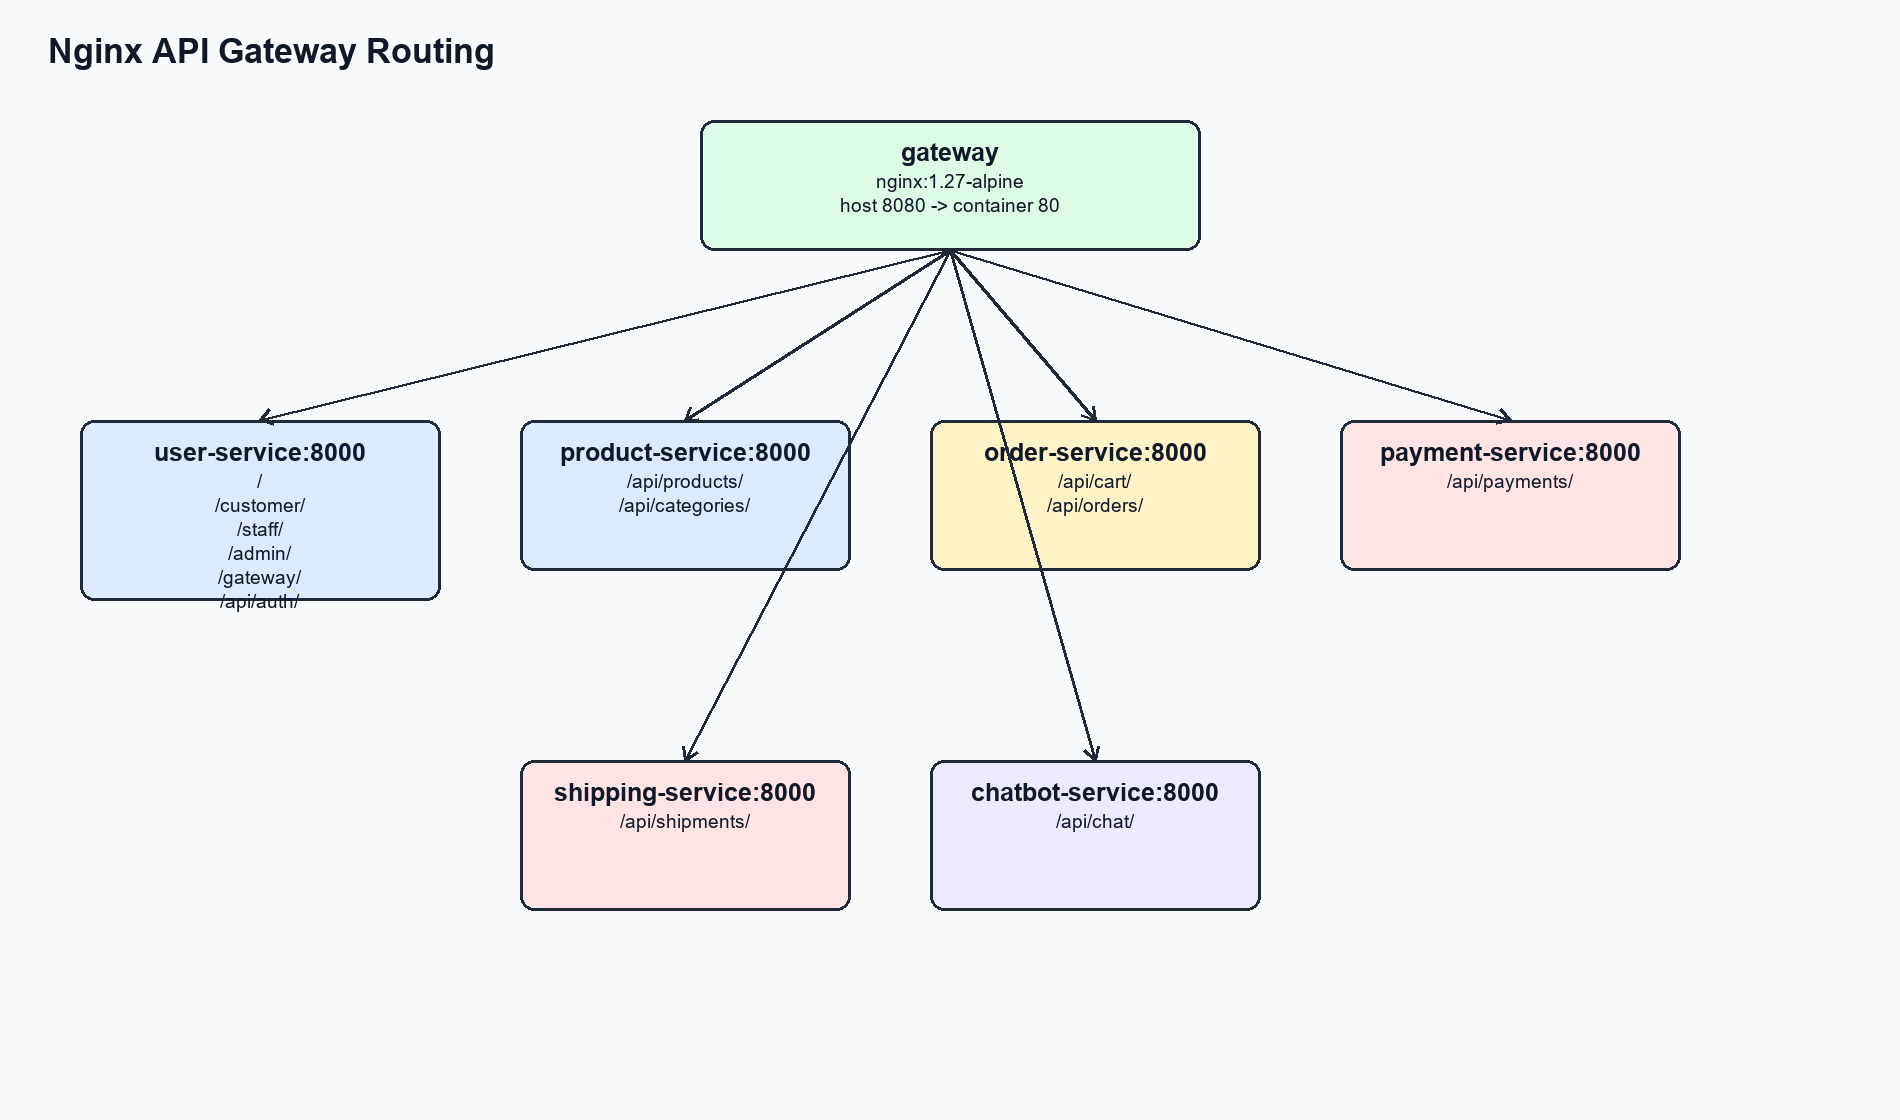
\includegraphics[width=0.98\linewidth]{final_diagram_images/ecom_gateway_routing.png}
\caption{Nginx API Gateway route mapping.}
\label{fig:ecom-gateway-routing}
\end{figure}

The gateway configuration is stored in \codepath{docker/gateway/nginx.conf}. The real routing uses Docker hostnames, not localhost ports, inside the Compose network.

\begin{lstlisting}[caption={Real Nginx gateway routing excerpt.}]
location / {
    set $target http://user-service:8000;
    proxy_pass $target;
}

location /customer/ {
    set $target http://user-service:8000;
    proxy_pass $target;
}

location /staff/ {
    set $target http://user-service:8000;
    proxy_pass $target;
}

location /api/auth/ {
    set $target http://user-service:8000;
    proxy_pass $target;
}

location /api/products/ {
    set $target http://product-service:8000;
    proxy_pass $target;
}

location /api/categories/ {
    set $target http://product-service:8000;
    proxy_pass $target;
}

location /api/cart/ {
    set $target http://order-service:8000;
    proxy_pass $target;
}

location /api/saved/ {
    set $target http://order-service:8000;
    proxy_pass $target;
}

location /api/compare/ {
    set $target http://order-service:8000;
    proxy_pass $target;
}

location /api/checkout/ {
    set $target http://order-service:8000;
    proxy_pass $target;
}

location /api/orders/ {
    set $target http://order-service:8000;
    proxy_pass $target;
}

location /api/staff/orders/ {
    set $target http://order-service:8000;
    proxy_pass $target;
}

location /api/analytics/ {
    set $target http://order-service:8000;
    proxy_pass $target;
}

location /api/internal/ {
    set $target http://order-service:8000;
    proxy_pass $target;
}

location /api/payments/ {
    set $target http://payment-service:8000;
    proxy_pass $target;
}

location /api/shipments/ {
    set $target http://shipping-service:8000;
    proxy_pass $target;
}

location /api/chat/ {
    set $target http://chatbot-service:8000;
    proxy_pass $target;
}
\end{lstlisting}

\subsection{Authentication and Authorization}

The system keeps two auth surfaces:

\begin{itemize}
    \item Django session authentication for browser UI routes under \codepath{/customer/*}, \codepath{/staff/*}, and \codepath{/admin/}.
    \item JWT API authentication for \codepath{/api/auth/register/}, \codepath{/api/auth/token/}, \codepath{/api/auth/token/refresh/}, and \codepath{/api/auth/me/}.
\end{itemize}

Internal APIs in \codepath{order\_service}, \codepath{payment\_service}, and \codepath{shipping\_service} validate service keys such as \codepath{ORDER\_SERVICE\_INTERNAL\_KEY}, \codepath{PAYMENT\_SERVICE\_INTERNAL\_KEY}, and \codepath{SHIPPING\_SERVICE\_INTERNAL\_KEY}.

\subsection{Communication Between Services}

The system uses synchronous REST. For example, \codepath{order\_service/orders/service\_clients.py} calls the payment service and shipping service through environment-driven URLs.

\begin{lstlisting}[language=Python,caption={Real internal service call pattern.}]
def create_pending_payment(order):
    return _request_json(
        "POST",
        f"{_payment_service_url()}/api/payments/",
        payload={
            "order_id": order.id,
            "user_id": order.user_id,
            "amount": order.total_amount,
            "status": "pending",
        },
        headers=_payment_headers(),
    )
\end{lstlisting}

\subsection{Docker Compose Deployment}

\begin{lstlisting}[caption={Real Docker Compose service excerpt.}]
gateway:
  image: nginx:1.27-alpine
  volumes:
    - ./docker/gateway/nginx.conf:/etc/nginx/nginx.conf:ro
  ports:
    - "8080:80"

product_service:
  build: ./services/product_service
  hostname: product-service
  ports:
    - "8001:8000"

order_service:
  build: ./services/order_service
  hostname: order-service
  environment:
    PAYMENT_SERVICE_URL: http://payment-service:8000
    SHIPPING_SERVICE_URL: http://shipping-service:8000
\end{lstlisting}

\subsection{End-to-End Checkout Flow}

\begin{enumerate}[label=\arabic*.]
    \item Customer submits checkout from \codepath{/customer/checkout/}.
    \item Nginx routes browser traffic to \codepath{user\_service}.
    \item \codepath{user\_service} signs and forwards checkout payload to \codepath{order\_service}.
    \item \codepath{order\_service} creates \codepath{Order}, \codepath{OrderItem}, and \codepath{OrderShipping} records.
    \item \codepath{order\_service} creates a pending payment in \codepath{payment\_service}.
    \item \codepath{order\_service} creates a pending shipment in \codepath{shipping\_service}.
    \item Payment confirmation updates payment status and order payment snapshot.
    \item Staff shipping update calls \codepath{shipping\_service} and synchronizes the current order shipping snapshot.
\end{enumerate}

\begin{figure}[H]
\centering
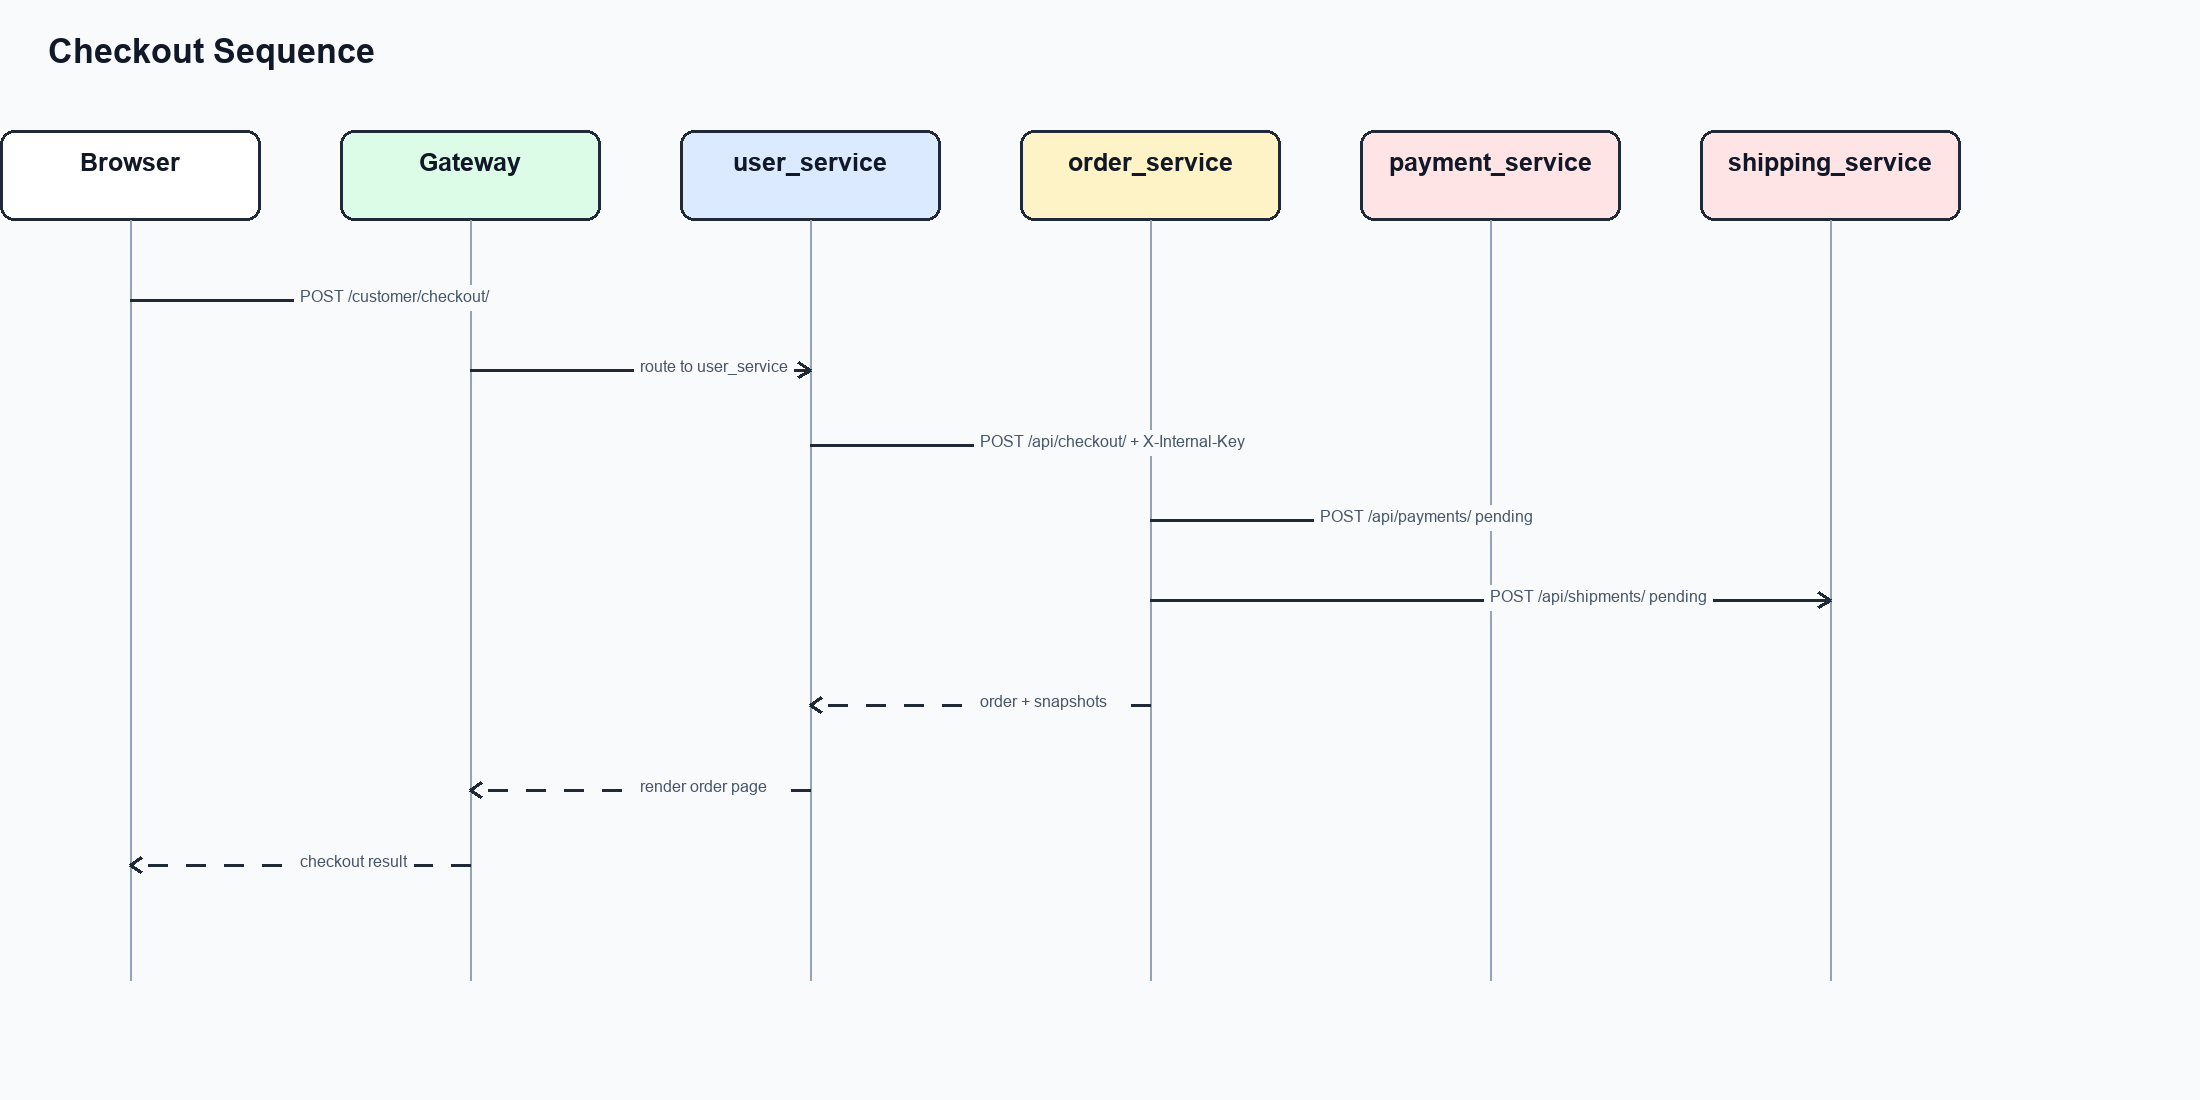
\includegraphics[width=0.98\linewidth]{final_diagram_images/ecom_checkout_sequence.png}
\caption{End-to-end checkout sequence for the real system.}
\label{fig:ecom-checkout-sequence}
\end{figure}

\subsection{Run and Verification Plan}

The practical verification commands are:

\begin{lstlisting}[caption={System run and smoke-check commands.}]
docker compose config --quiet
docker compose up --build -d
docker compose ps
Invoke-WebRequest http://localhost:8080/customer/login/
Invoke-WebRequest http://localhost:8080/api/categories/
Invoke-WebRequest http://localhost:8080/api/chat/reply/ -Method Post `
  -ContentType 'application/json' -Body '{"message":"goi y laptop hoc tap"}'
\end{lstlisting}

Relevant service tests should be run with \codepath{python manage.py test} in each touched service when service code changes. This essay update changes documentation and generated diagram artifacts only, so the most important checks are LaTeX compilation and Docker/gateway smoke checks.

\subsection{System Evaluation}

\subsubsection{Advantages}

\begin{itemize}
    \item The API Gateway hides internal service URLs and keeps \codepath{8080} as the public entrypoint.
    \item Product, order, payment, shipping, user, and chatbot responsibilities are separated by business capability.
    \item MySQL and PostgreSQL are selected service by service instead of forcing one database for the whole project.
    \item AI dependencies and artifacts stay isolated in \codepath{chatbot\_service}.
\end{itemize}

\subsubsection{Remaining Risks}

\begin{itemize}
    \item The system still uses synchronous REST calls, so checkout depends on downstream payment and shipping service availability.
    \item There is no distributed tracing stack yet, so multi-service debugging still depends on container logs.
    \item Cart is a logical bounded capability inside \codepath{order\_service}, not an independently scalable container.
    \item LLM calls require external API keys; fallback behavior is implemented, but generated answer quality depends on runtime configuration.
\end{itemize}

\subsection{Conclusion}

The complete system satisfies the core microservice evidence required by the report: real Docker Compose deployment, Nginx gateway routing, database-per-service design, Django models and APIs per service, checkout orchestration, and a working AI consultation service integrated into the e-commerce flow.

\section*{Final Conclusion}
\addcontentsline{toc}{section}{Final Conclusion}

This essay follows the lecturer's structure: it first explains monolithic architecture, microservices, and DDD; then it develops the real e-commerce microservice design from the current repository; then it presents the AI service for product consultation; and finally it describes the complete system architecture, gateway, security, communication, Docker deployment, workflow, and evaluation.

The healthcare system appears only as the case study in Section 1.4 for practicing DDD decomposition. The main project remains the e-commerce microservices system with AI recommendation and chatbot consultation.

\section*{References}
\addcontentsline{toc}{section}{References}

\begin{enumerate}[label={[\arabic*]}]
    \item E. Evans, \textit{Domain-Driven Design: Tackling Complexity in the Heart of Software}. Addison-Wesley, 2003.
    \item S. Newman, \textit{Building Microservices: Designing Fine-Grained Systems}, 2nd ed. O'Reilly Media, 2021.
    \item M. Fowler and J. Lewis, ``Microservices: a definition of this new architectural term,'' 2014.
    \item C. Richardson, \textit{Microservices Patterns}. Manning Publications, 2018.
    \item Django Software Foundation, ``Django Documentation.'' Official documentation.
    \item Django REST Framework, ``Django REST Framework Documentation.'' Official documentation.
    \item Neo4j, ``Neo4j Graph Database Documentation.'' Official documentation.
    \item scikit-learn developers, ``scikit-learn Documentation.'' Official documentation.
\end{enumerate}

\appendix

\section{Implementation Evidence Used}

This appendix records the concrete project evidence used to replace the earlier generic examples:

\begin{itemize}
    \item Root folder: \codepath{c:/Users/nguye/Desktop/kiemtra01}.
    \item Runtime configuration: \codepath{docker-compose.yml}.
    \item Gateway routing: \codepath{docker/gateway/nginx.conf}.
    \item Product model/API/seed data: \codepath{services/product\_service/catalog/models.py}, \codepath{urls.py}, \codepath{seed\_data.py}.
    \item User auth and UI routes: \codepath{services/user\_service/customer/api\_auth.py}, \codepath{customer/urls.py}, \codepath{staff/urls.py}.
    \item Commerce state: \codepath{services/order\_service/orders/models.py}, \codepath{urls.py}, \codepath{service\_clients.py}.
    \item Payment and shipping lifecycle: \codepath{services/payment\_service/payments/models.py}, \codepath{services/shipping\_service/shipments/models.py}.
    \item AI service: \codepath{services/chatbot\_service/chatbot/models.py}, \codepath{services.py}, \codepath{behavior\_ai.py}, \codepath{behavior\_graph.py}, \codepath{rag\_kb.py}.
    \item AI artifacts and screenshots: \codepath{services/chatbot\_service/chatbot/artifacts/} and \codepath{docs/evidence/screenshots/}.
    \item Final report diagrams: \codepath{EssayV1/final\_diagram\_images/}. PNG diagrams are generated by \codepath{EssayV1/generate\_ecom\_diagrams.py}; detailed class and data-model diagrams are exported from Visual Paradigm as SVG files.
\end{itemize}

\clearpage
\section{Classmate Review Table}

This table is prepared for classmates to review the report during the final classroom discussion.

\begin{table}[H]
\centering
\caption{Classmate review table.}
\label{tab:classmate-review}
\small
\setlength{\tabcolsep}{3pt}
\renewcommand{\arraystretch}{1.2}
\begin{tabular}{|L{0.14\linewidth}|C{0.12\linewidth}|L{0.52\linewidth}|C{0.07\linewidth}|C{0.07\linewidth}|}
\hline
\textbf{Name} & \textbf{ID} & \centering\arraybackslash\textbf{Assessment Notes} & \textbf{Score} & \textbf{Sign.}\\
\hline
\rule{0pt}{2.05cm} & & & &\\
\hline
\rule{0pt}{2.05cm} & & & &\\
\hline
\rule{0pt}{2.05cm} & & & &\\
\hline
\rule{0pt}{2.05cm} & & & &\\
\hline
\rule{0pt}{2.05cm} & & & &\\
\hline
\rule{0pt}{2.05cm} & & & &\\
\hline
\rule{0pt}{2.05cm} & & & &\\
\hline
\rule{0pt}{2.05cm} & & & &\\
\hline
\rule{0pt}{2.05cm} & & & &\\
\hline
\rule{0pt}{2.05cm} & & & &\\
\hline
\end{tabular}
\setlength{\tabcolsep}{6pt}
\renewcommand{\arraystretch}{1}
\normalsize
\end{table}

\end{document}
